% !TeX program = lualatex
% !TeX encoding = utf8
% !TeX spellcheck = uk_UA

\documentclass{LabBook}
%\usepackage{lua-widow-control}
\graphicspath{{pic/}}

\addbibresource{\jobname.bib}
\edef\infile{ExpData.dat}
\edef\outfile{FitParam.dat}

% Виклик скрипта GNUPLOT для апроксимації даних
\input{|gnuplot -persist -c GnuFit.gp \infile\space\outfile}

% Виклик скрипта PYTHON для апроксимації даних
%\input{|python PyFit.py \infile\space \outfile}

%============================= Заголовок документу======================================%
\title{Обробка результатів експерименту}
\def\subtitle{}

%% !TeX program = lualatex
% !TeX encoding = utf8
% !TeX spellcheck = uk_UA
% !TeX root =../EMProblems.tex

%========================================================================================================
%
%									      Палітурка
%
%========================================================================================================

% ---------------------------------------- Кольори секцій -----------------------------------------------
\definecolor{themecolordark}{RGB}{34,102,101}
\definecolor{themecolorlight}{RGB}{153,168,167}
\definecolor{titlebgdark}{RGB}{0,103,102}
\definecolor{titlebglight}{RGB}{191,233,251}

\newcommand{\CoverPage}{
	\begin{alwayssingle}
		\begin{center}
			\begin{flushright}\bfseries\sffamily
				\MakeUppercase{Міністерство освіти і науки України}\\
				КПІ ім. Ігоря Сікорського\\
			\end{flushright}
			\begin{tcolorbox}[titlepagestyle,
					toprule=0.10cm,
					bottomrule=0.10cm,
					overlay={%
						\node (picture) at ([xshift=4cm]frame.west) {
\includegraphics{logo_PTI}};
					}
			]%
			\begin{flushright}
				\large\bfseries\color{white}Фізико-технічний інститут
			\end{flushright}
			\end{tcolorbox}

			\vspace*{15em}

			\begin{tcolorbox}[
				titlepagestyle,
				toprule=0.15cm,
				bottomrule=0.15cm,
				top=1.3cm,
				bottom=0.7cm,
				overlay={%
				\node[%
							fill=white,
							rounded corners = 15pt,	
							draw=themecolorlight,
							line width=0.15cm,
							inner sep=0pt,
							text width=17cm,
							minimum height=2cm,
							align=center,
							%anchor=east,
							font=\sffamily\bfseries\large
						] (title) at (frame.north) {С.~М. Пономаренко
					};
				}
			]
			\centering
			\Huge\sffamily\bfseries\textcolor{white}{\realtitle}\\
			\huge\sffamily\bfseries\textcolor{white}{\subtitle}
			\end{tcolorbox}	
			\vfill
%		 	\begin{Large}\color{themecolordark!90!black}
%			\begin{gather*}
%				\frac{\partial F^{\mu\nu}}{\partial x^\nu} =                                                                                -\frac{4\pi}{c}j^\mu \\
%				\frac{\partial F^{\mu\nu}}{\partial x^\alpha} + \frac{\partial F^{\mu\alpha}}{\partial x^\nu} +\frac{\partial F^{\alpha\mu}}{\partial x^\nu}  = 0.
%			\end{gather*}
%			\end{Large}
			\vfill
			\begin{tcolorbox}[titlepagestyle,
					toprule=0.10cm,
					bottomrule=0.10cm]
				\begin{center}\color{white}\bfseries\normalsize
					\MakeUppercase{Київ~2021} \\
%					КПІ ім. Ігоря Сікорського \\
%					\the\year
				\end{center}			       	
			\end{tcolorbox}
		\end{center}
		\clearpage
	\end{alwayssingle}
\setcounter{page}{1}	
}


%========================================================================================================
%
%									      Титульна сторінка
%
%========================================================================================================

\renewcommand\maketitle{
	\begin{alwayssingle}
		\begin{center}
				\MakeUppercase{Міністерство освіти і науки України}
				
				\bigskip
				\MakeUppercase{Національний технічний університет України}\\
				<<КИЇВСЬКИЙ ПОЛІТЕХНІЧНИЙ ІНСТИТУТ \\ імені ІГОРЯ СІКОРСЬКОГО>>
				\vspace*{150pt}
		
%				{\large С.~Пономаренко,
%						Ю.~О.~Тараненко
%						}
%				\vspace*{50pt}
			
				{\Huge\sffamily\bfseries\realtitle}\\[1em]
				{\huge\sffamily\bfseries\subtitle}	
			
			\vspace*{50pt}
			\begin{center}\itshape
                Рекомендовано Методичною радою КПІ ім. Ігоря Сікорського як навчальний посібник для здобувачів ступеня бакалавра за освітньою програмою <<Прикладна фізика>> спеціальності 105 Прикладна фізика та наноматеріали 
%				Методичні вказівки до виконання лабораторних робіт за темою <<Змінний струм>> з навчальної дисципліни <<Електрика та магнетизм>> для студентів, які навчаються за спеціальністю 105 <<Прикладна фізика та наноматеріали>>
			\end{center}

			\vfill
			\begin{center}
				\MakeUppercase{Київ} \\
				КПІ ім. Ігоря Сікорського \\
				2020
			\end{center}			       	
		\end{center}
		\clearpage
	\end{alwayssingle}	
}


%========================================================================================================
%
%									      Друга сторінка
%
%========================================================================================================
\newcommand\makeinfopage{
	\begin{alwayssingle}
		\noindent%	
        \begin{minipage}[t]{\textwidth}
                \realtitle: \subtitle\ [Електронний ресурс] : навч. посіб. для студ. спеціальностей
                105 <<Прикладна фізика та наноматеріали>> / КПІ ім. Ігоря Сікорського; уклад.  С.~М. Пономаренко; КПІ ім. Ігоря Сікорського.~--- Електронні текстові дані
            (1 файл: 3.30~МБ). – Київ : КПІ ім. Ігоря Сікорського, 2020. --- \the\numexpr\getpagerefnumber{LastPage}~с.
        \end{minipage}
        \vspace*{2em}
		\begin{center}\itshape\small
				Гриф надано Методичною радою КПІ ім. Ігоря Сікорського (протокол № 4 від 10.12.2020 р.) за поданням Вченої ради Фізико-технічного інституту (протокол №11/2020 від 26.11.2020 р.)
		\end{center}
		\begin{center}
			Електронне мережне навчальне видання
			%\par {Версія від~\href{http://www.istpravda.com.ua/dates}{\today}} \par\else \par  \fi
		\end{center}
		\begin{center}\bfseries
    		\LARGE\sffamily\realtitle\\
   			\Large\sffamily\subtitle
   		\end{center}

		\vfill\noindent%
        \begin{minipage}[t]{0.2\linewidth}
            	\begin{flushleft}
                    Укладачі:
                \end{flushleft}
        \end{minipage}\hfill
        \begin{minipage}[t]{0.78\linewidth}
		\begin{flushleft}
			\href{http://apd.ipt.kpi.ua/blog/author/183}{\itshape Пономаренко Сергій Миколайович}, к.ф.-м.н., доцент
		\end{flushleft}
        \end{minipage}

        \vspace*{2em}
		\noindent%
        \begin{minipage}[t]{0.2\linewidth}
            	\begin{flushleft}
                    Відповідальний редактор:
                \end{flushleft}
        \end{minipage}\hfill
        \begin{minipage}[t]{0.78\linewidth}
                к.ф.-м.н., доцент \href{http://ipt.kpi.ua/smirnov}{Смирнов С.~О.}
        \end{minipage}

        \vspace*{2em}
		\noindent%
%        \begin{minipage}[t]{0.2\linewidth}
%            	\begin{flushleft}
%                    Рецензент:
%                \end{flushleft}
%        \end{minipage}\hfill
%        \begin{minipage}[t]{0.78\linewidth}
%                \href{http://apd.ipt.kpi.ua/blog/author/19}{Я.~Д.~Кривенко-Еметов}, к.ф.-м.н., доцент кафедри прикладної фізики, Фізико-технічного інституту КПІ ім. Ігоря Сікорського
%        \end{minipage}

        \vfill

		Розглянуто зміст, основні складові та порядок виконання лабораторних робіт за темою <<Змінний струм>> з дисципліни <<Електрика та магнетизм>>. 

		Для студентів фізико-технічного інституту КПІ ім. Ігоря Сікорського, які навчаються за спеціальністю 105~<<Прикладна фізика та наноматеріали>>.
		
		\vfill
				
%		\begin{flushleft}\small
%			Ілюстративний матеріал підручника підготовлений за допомогою пакету \href{http://pgf.sourceforge.net}{TikZ/Pgf}. Верстка тексту проведена в видавничій системі \LaTeXe{} (компілятор Lua\LaTeX) на базі системи комп'ютерної верстки \TeX{} (Збірка  \href{https://www.tug.org/texlive/}{\TeX Live~\the\year}) з використанням оболонки \href{https://www.texstudio.org}{\TeX Studio}.
%		\end{flushleft}	
	\begin{flushright}
        \textcopyright{} С.~М. Пономаренко, 2021 р.
    \end{flushright}
		\newpage%
	\end{alwayssingle}
}




\begin{document}
%\CoverPage
\maketitle
%\makeinfopage
\tableofcontents
\clearpage
\pagestyle{main}


\chapter{Що таке похибки і навіщо їх оцінювати?}

Результати вимірювання мають певний ступінь невизначеності. Процес оцінки невизначеності, пов'язаної з результатом вимірювання, називають аналізом невизначеностей.
%, або аналізом похибок\footnote{В англомовній літературі невизначеності називаються як <<uncertainty>>, або ж як <<errors>>. У вітчизняній літературі зазвичай користуються терміном <<похибка>>.}.

Коли ми представляємо результат виміряної величини, він повинен включати оцінку рівня впевненості, з якою отриманий цей результат. Правильне звітування про експериментальний результат разом із його невизначеністю дозволяє іншим людям робити судження про якість експерименту, а також полегшує порівняння з іншими подібними значеннями або теоретичним прогнозом. Без оцінки невизначеності неможливо відповісти на основне наукове запитання: <<\emph{Чи узгоджується мій результат з теоретичним прогнозом чи результатами інших експериментів?}>> Це питання є фундаментальним для вирішення питання про підтвердження чи спростування наукової гіпотези.

Коли ми робимо вимірювання, ми зазвичай припускаємо, що існує деяке \emph{точне} або \emph{істинне значення вимірюваної величини}. Хоча ми, можливо, ніколи не дізнаємося, чому дорівнює це значення, але ми намагаємося якомога точніше його встановити в  міру своїх можливостей, використовуючи наявний час і ресурси.

%Не буде перебільшенням сказати, що експериментальний результат, пред'явлений без зазначення такого діапазону --- безглуздий.

%\begin{More}
%В сучасній метрології --- термін <<похибка>> та термін <<невизначеність>> є дещо відмінними. Поняття <<похибка>> результату виміру показує відхилення результату вимірювання від істинного (дійсного) значення вимірюваної величини. Проте похибка не може бути точно відома, оскільки істинне  значення завжди невідоме. Суть процесу вимірювань --- порівняння вимірюваної величини із мірою. При цьому в практичній метрології використовують два прийоми оцінки якості вимірів: пряме порівняння вимірюваної величини з мірою (тобто з умовно істинним або дійсним значенням), що відтворюється за допомогою еталона, робітника або стандартного зразка; оцінка шляхом розрахунку, заснованого на апріорному знанні деяких характеристик методу, досліджуваного об'єкта, засобів та умов вимірювань. У практиці, що склалася, в галузі метрології і те, й інше називають похибкою вимірів. Введення "концепції невизначеності" дозволяє розділити ці два прийоми оцінки
%якості вимірів.
%
%У «концепції невизначеності» точність результату виміру характеризується його невизначеністю. Фактично концепція побудована на постулат: результат виміру - випадкова величина. Основним документом міжнародного рівня, який реалізує «концепцію невизначеності», є міжнародна рекомендація GUM [3], розроблена в 1993 російською мовою зазначена рекомендація з'явилася в 1999 [4]. В Україні практичні рекомендації щодо застосування [4] представлені у Посібнику [5]. Відповідно до «Міжнародного словника основних та загальних термінів в області метрології» [6], невизначеність вимірів – це параметр, пов'язаний із результатом вимірювання та характеризує розкид значень, які могли б бути обґрунтовано приписані вимірюваній величині. Невизначеність вимірювань, як параметр, характеризує розсіювання множини можливих значень величин, а не похибка конкретного результату виміру [7]. Методи обчислення невизначеності, як і методи оцінювання похибки, засновані на тих самих методах математичної статистики.
%Подібними для обох підходів є і послідовність дій обчисленні похибки та невизначеності вимірювань
%\end{More}

Оскільки ми проводимо вимірювання різними методами, або навіть коли робимо кілька вимірювань за допомогою одного й того ж методу, ми постійно отримуємо трохи різні результати. Тож, як саме ми повідомимо про наші висновки для найкращої оцінки цього невловимого істинного значення? Найпоширеніший спосіб показати діапазон значень, який, на нашу думку, \emph{ймовірно} включає справжнє значення. І слово \emph{ймовірно} тут важливе.


Будь-яке число, яке видає нам експеримент~--- це результат вимірювання\footnote{Це знаменита фраза капітана <<Очевидність>>}. Вимірювання проводиться приладом, і це або безпосередні покази приладу, або результат обробки цих показів. В першому випадку вимірювання називаються \emph{прямими}, в другому --- \emph{непрямими}.

%І в тому, і в іншому випадку отриманий результат вимірювання величини неідеальний, ніхто не розраховує отримати його її істинне значення. Тому необхідно вказати, наскільки отриманий результат може бути близьким до істинного значення, тобто вказати яка точність вимірювання. А тому грамотний фізик повинен не тільки пред'явити чисельний результат вимірювання, а й зобов'язаний вказати \emph{приблизну} похибку вимірювання. Не буде перебільшенням сказати, що чисельний експериментальний результат, пред'явлений без зазначення будь-яких похибок, безглуздий.

Розглянемо, для прикладу, результат зважування якогось предмета, що виглядає як
\begin{equation}\label{}
	m = 100 \pm 5~\text{грам}.
\end{equation}

У побутовій ситуації такий запис часто інтерпретується так, немов справжня маса гарантовано лежить в цьому діапазоні і ні в якій мірі не може бути $94$ або $106$ грам. Науковий запис має на увазі не це. І тут ми повертаємось до слова <<\emph{ймовірно}>>. Цей запис означає, що ми не знаємо істинну масу точно, вона може бути і $101$ грам, і $96$ грам, а може бути і всі $108$ грам. На скільки далеко істинне значення може відхилятись від середнього? Теорія ймовірностей дає нам інструмент, який дозволяє визначити таку ймовірність, про ще ми поговоримо згодом.

Вимога наводити результат з відповідною точністю стосується не лише остаточного результату експерименту, воно стосується  також і тих величин, що вимірюються в ході цього вимірювання. Адже рідко бувають такі прості експерименти, в яких остаточна величина вимірювалася би безпосередньо. Зазвичай доводиться прямо вимірювати цілий ряд проміжних величин, які лише в комбінації дають необхідний результат. При цьому похибка остаточного результату визначається похибками прямих вимірюваннях проміжних величин. Загалом, ці похибки по-різному впливають на остаточну. Остання буде мінімальною, якщо розподілити наявні ресурси часу, приладів і терпіння так, щоб зменшити ті помилки і які дають найбільший вклад в остаточну помилку.

%Поняття похибки вимірювання відіграє далеко по другорядну роль в експерименті. Навпаки, воно має пряме відношення до таких питань, як мета експерименту, його метод і значущість його результатів.

Перейдемо тепер до означень.

Абсолютна похибка вимірювання --- це відхилення виміряного значення величини від її істинного значення $x$:
\begin{equation}\label{eq:delta}
	\delta x = x_\text{вимір} - x.
\end{equation}

Крім абсолютної похибки $\delta x$, часто буває важливо знати відносну похибку $\delta x$, яка дорівнює відношенню
абсолютної похибки до значення вимірюваної величини:
\begin{equation}\label{eq:reldelta}
	\varepsilon = \frac{\delta x}{x}.
\end{equation}

Як випливає з \eqref{eq:delta} і \eqref{eq:reldelta}, для того, щоб знайти абсолютну я відносну похибку вимірювань, потрібно знати не тільки виміряне, а й істинне значення величини, яка нас цікавить. Але якщо істинне значення відоме, то навіщо робити вимірювання? Тому формули \eqref{eq:delta} і \eqref{eq:reldelta}, що визначають величину похибок, не мають практичного сенсу. В практичних вимірюваннях похибки можна лише \emph{оцінити}.


%\chapter{Прямі та непрямі вимірювання}
%
%
%Якщо величина $x$ вимірюється безпосередньо приладом, то це пряме вимірювання. Однак, є багато величин, які прямо виміряти не можна, а можна лише розрахувати за формулою. В цю формулу входять величини, що вимірюються прямо. Такі, обчислювані величини називаються непрямими вимірами, а похибки таких величин визначаються похибками величин, що входять  у формулу.
%
%У загальному випадку абсолютна (і відносна) похибка величини, що розраховується визначається з правил диференціювання функції $Y$ багатьох змінних $x_1, x_2, \ldots, x_n$:
%\begin{equation}\label{}
%    \Delta Y =
%\end{equation}

\chapter{Систематичні та статистичні похибки}


Похибки розділяються на два типи: \emph{статистичні} і \emph{систематичні}. Мета такого поділу --- дати чітке розуміння того, що саме обмежує точність цього конкретного вимірювання, а отже, за рахунок чого цю точність можна покращити в майбутньому.

Систематичними похибками називаються такі похибки, які залишаються незмінними при вимірюваннях. Серед них можна виділити: \emph{поправки} (постійні впливи чогось на прилади), \emph{похибки невідомого походження} (недостатньо розроблена теорія, складний експеримент) та \emph{клас точності приладів}. Найчастіше клас точності приладів вважається основним джерелом систематичних помилок.

У електровимірювальних приладах зазвичай є класи від $0.05$ до $4$. Що це означає? Якщо, клас точності приладу, наприклад, дорівнює $0.5$ а шкала має $100$ поділок, то це означає, що покази приладу даються не точніше, ніж 0.5 \% від шкали, тобто, $0.5$ поділки.

Статистичними похибками (або випадковими) називають такі похибки, які змінюються від досліду до досліду, носять випадковий характер і можуть бути як додатними такі від'ємними.

Випадкові похибки завжди присутні в експериментах завдяки різним неконтрольованим впливам на прилади і за відсутністю систематичних помилок, вони є причиною розкиду повторних вимірювань навколо істинного значення (рис.~\ref{pic:stat}). Якщо в дослідах присутня також систематична похибка, то результати вимірювань будуть розкидані навколо не істинного, а зміщеного значення (рис.~\ref{pic:system}).

\begin{figure}[h!]\centering

	\begin{subfigure}[b]{0.45\linewidth}\centering
		\begin{tikzpicture}[
				font=\sffamily,
				every node/.style={
						font=\sffamily,
					},]
			\draw [-latex] (3,0) -- (7,0) node[right] {$x$};
			\foreach \x in {4.7,4.9,5,5.1,5.3} {
					\draw (\x,7pt) -- (\x,-7pt);
				}
			% \node[pin={[pin distance=0.5cm, pin edge={red,stealth-}]above:{$\left\langle x \right\rangle$}}] at (5,0) {};
			\node[pin={[pin distance=0.5cm, pin edge={red,stealth-}]below:{$x$}}] at (5.1,0) {};
		\end{tikzpicture}
		\caption{}
		\label{pic:stat}
	\end{subfigure}
	\begin{subfigure}[b]{0.45\linewidth}\centering
		\begin{tikzpicture}[
				font=\sffamily,
				every node/.style={
						font=\sffamily,
					},]
			\draw [-latex] (3,0) -- (7,0) node[right] {$x$};
			\foreach \x in {4.7,4.9,5,5.1,5.3} {
					\draw (\x,7pt) -- (\x,-7pt);
				}
			% \node[pin={[pin distance=0.5cm, pin edge={red,stealth-}]above:{$\left\langle x \right\rangle$}}] at (5,0) {};
			\node[pin={[pin distance=0.5cm, pin edge={red,stealth-}]below:{$x$}}] at (6,0) {};
		\end{tikzpicture}
		\caption{}
		\label{pic:system}
	\end{subfigure}
	\caption{}
	\label{pic:stat+syst_error}
\end{figure}

Статистичні (або випадкові) помилки можна зменшити збільшуючи число вимірювань, а оцінити їх можна використовуючи методи математичної статистики. При наявності ж систематичних помилок, ви можете повторювати якесь вимірювання на приладі мільйони разів, але якщо у нього <<збитий приціл>>, то ви систематично будете отримувати значення, що відрізняється від істинного. Систематична похибка вказує наскільки прилад <<бреше>>, і якщо це ми добре знаємо, то тим самим зможемо скоригувати його покази і усунути цю похибку. Однак, якщо ми не знаємо, а гірше того, навіть не підозрюємо про наявність систематичної помилки, то це може призвести до небезпечних наслідків. Загальних рецептів по їх виявленню не має, тому експериментатору треба самостійно спланувати експеримент так, щоб усунути, або зменшити ці похибки.


\chapter{Як оцінюються похибки?}






\section{Оцінка систематичних похибок}




Систематичні похибки --- це такі похибки, які залишаються постійними (за величиною і знаком) або закономірно змінюються при повторних вимірюваннях. В результаті існування таких похибок середня вимірювана величина відхиляється від очікуваної на деяку постійну величину.
Розрізняють чотири типи систематичних похибок:
\begin{itemize}
\item Похибки відомої природи і їх величини можуть бути визначені. Для усунення таких похибок вводяться поправки. Так, наприклад, при вимірюванні довжини тіла за допомогою лінійки необхідно врахувати поправку на теплове розширення як самого тіла, так і лінійки при заданій температурі.
\item Похибки невідомої природи. Наприклад, при визначенні густини тіла шляхом вимірювання маси та об’єму при наявності порожнин у тілі буде допускатися систематична похибка, усунути яку можна лише, застосувавши інший спосіб вимірювання даної величини.
\item Похибки, пов’язані із властивостями досліджуваного об’єкта, наприклад, із не ідеальністю його форми, що призведе до похибки у вимірюванні його розмірів.
\item Інструментальні похибки --- похибки відомої природи, але невідомої величини, які зумовлені неточністю самих вимірювальних приладів.
\end{itemize}

Оскільки в лабораторних роботах найчастіше доводиться зіштовхуватися із інструментальними систематичними похибками, то саме цей клас похибок розглянемо детальніше.

\textbf{Інструментальні похибки} (похибки приладів) обумовлені багатьма причинами, пов’язаними із конструкцією приладів, якістю їх виготовлення, ретельністю налаштування, умовами застосування і т.д.

Так, наприклад, неможливо знайти рулетку з ідеально точним розбиттям шкали, абсолютно точні гирі, ідеально рівноплечі важелі.

Інструментальні похибки можна встановити при порівнянні показів даного вимірювального приладу із показами більш точного. Така процедура називається \emph{повіркою приладу}.

\subsection{Визначення та врахування систематичних похибок. Клас точності приладів}


Похибки вимірювальних засобів --- це гранично допустимі абсолютні або відносні похибки, що встановлюються державними відділами стандартів для виробництв, що виготовляють вимірювальні засоби. Ці граничні похибки вказані на приладах або в їхніх паспортах. Наприклад, в паспорті до гирь для технічних аналізів масою 10, 20, 50 та 100 мг вказана їхня гранична похибка $\Delta m_\text{інст} = 1$~мг.
Точність електровимірювальних приладів (амперметрів, вольтметрів і т.д.), деяких мір (магазинів опорів, індуктивностей, електроємностей і т.д.) та ряду інших приладів характеризується класом точності $k$.
Клас точності --- це число, рівне вираженому у відсотках відношенню абсолютної похибки приладу $\Delta _\text{інст}$ до  максимального значення вимірюваної ним величини $x_{\max}$:

\begin{align*}
   k= \frac{\Delta_\text{інст}}{x_{\max}} \cdot 100\%
\end{align*}



Для електровимірювальних приладів  можливі 8 класів точності $ 0.02 $; $ 0.05 $; $ 0.1 $; $ 0.2 $; $ 0.5 $; $ 1.0 $; $ 1.5 $; $ 2.5 $; $ 4.0 $, що  вказуються  на  шкалі цих приладів або в їхньому паспорті.

Знаючи клас точності можна легко знайти максимальну абсолютну інструментальну похибку:

\begin{align*}
  \Delta_\text{інст} =  \frac{k \cdot x_{\max}}{100}
\end{align*}

Наприклад, припустимо, що в дослідах використовується амперметр, клас точності якого  $k = 0.5$, границя вимірювання ---$  50 $ mA. Абсолютна похибка приладу:

\begin{align*}
 \Delta I_\text{інст} =  \frac{0.5 \cdot 50 \ \text{мА}}{100}=0.25\ \text{мА}
\end{align*}


\begin{Warning}
Звернемо увагу, що похибка в $ 0.25 $~мA складає невелику долю від вимірювального струму ($ 0.5 $ \%) лише при умові відхилення стрілки амперметра на усю шкалу. Навпаки, при відхиленні стрілки приладу, наприклад, на половину шкали під час вимірювання меншого значення струму значення відносної похибки зросте і становитиме: $\frac{{\Delta I}}{I} = \frac{0.25\ \text{мА}}{25\ \text{мА}} \cdot 100 \ \%  = 1\ \% $ . При вимірювання це менших значень струму цим амперметром відносна похибка буде ще зростати. Таким чином, при проведенні вимірювання з великою точністю необхідно вибирати такий прилад, у якому вимірювальний струм призведе до відхилення стрілки більше ніж на половину шкали.
\end{Warning}


При невідомій точності приладу користуються таким наближеним правилом: якщо вимірювання проводяться шляхом порівняння вимірюваної величини із якою-небудь шкалою, то точність приладу визначається половиною ціни найменшої поділки шкали приладу (лінійка, термометр, секундомір). Якщо вимірювання проводяться приладом із ноніусом (штангенциркуль), то точність приладу приймається рівною різниці між ціною однієї поділки приладу та однієї поділки ноніуса.



\section{Оцінка статистичних похибок}


Випадкові похибки, як уже було сказано вище, є причиною розкиду повторних вимірювань навколо істинного значення (рис.~\ref{pic:error}). Слід застерегти, що слово <<випадкові>> зовсім не означає, що  їх величина може бути якою завгодно, у випадкових подій також є свої закони. Наприклад, якщо прово\-дить\-ся серія експериментів і результати <<кучно лягають>> біля свого середнього значення (рис.~\ref{pic:low}), то можна казати, що істинне значення $x$ скоріше за все має бути досить близькою до  $\left\langle x \right\rangle$, тоді як в ситуації зображеній на рис.~\ref{pic:huge} різниця може виявитись більшою. Точно сказати, де саме буде це істинне значення ми не можемо, але можна вказати з якою ймовірністю воно опиниться в тому чи іншому інтервалі навколо $\left\langle x \right\rangle$.

Тому адекватною мовою для опису похибок --- є мова ймовірності.
%Поки поняття похибки доволі туманне, але спробуємо дати чітке означення. Для цього нам знадобиться поняття розподілу і центральна гранична теорема.

\begin{figure}[h!]\centering
	\begin{subfigure}[b]{0.45\linewidth}\centering
		\begin{tikzpicture}[
				font=\sffamily,
				every node/.style={
						font=\sffamily,
					},]
			\draw [-latex] (3,0) -- (7,0) node[right] {$x$};
			\foreach \x in {4.7,4.9,5,5.1,5.3} {
					\draw (\x,7pt) -- (\x,-7pt);
				}
			\node[pin={[pin distance=0.5cm, pin edge={red,stealth-}]above:{$\left\langle x \right\rangle$}}] at (5,0) {};
			\node[pin={[pin distance=0.5cm, pin edge={red,stealth-}]below:{$x$-?}}] at (5.1,0) {};
		\end{tikzpicture}
		\caption{}
		\label{pic:low}
	\end{subfigure}
	\begin{subfigure}[b]{0.45\linewidth}\centering
		\begin{tikzpicture}[
				font=\sffamily,
				every node/.style={
						font=\sffamily,
					},]
			\draw [-latex] (3,0) -- (7,0) node[right] {$x$-?};
			\foreach \x in {3.7,4.5,5,5.6,6, 6.3} {
					\draw (\x,7pt) -- (\x,-7pt);
				}
			\node[pin={[pin distance=0.5cm, pin edge={red,stealth-}]above:{$\left\langle x \right\rangle$}}] at (4.68,0) {};
			\node[pin={[pin distance=0.5cm, pin edge={red,stealth-}]below:{$x$-?}}] at (4,0) {};
		\end{tikzpicture}
		\caption{}
		\label{pic:huge}
	\end{subfigure}
	\caption{Серія прямих вимірювань величини $x$. Чим точніше виконуються експерименти, тим менше статистична похибка (<<кучніше результати>>).}
	\label{pic:error}
\end{figure}



\section{Оцінка похибок прямих вимірювань}


%Для того, щоб дати чітке означення похибки вимірювання треба скористатись центральною граничною теоремою. Як це зробити? Поступово підійдемо до цього поняття.

Нехай, $n$ вимірювань деякої величини дало нам сукупність значень:
\begin{equation}\label{selection}
	x_1, x_2, \ldots, x_n.
\end{equation}

Зазвичай, на практиці ніхто не виконує нескінченну кількість вимірювань, в навчальних лабораторіях ця кількість сягає $n = 10 \ldots 50$. Число $n$ значень називається \emph{вибіркою}.

На основі вимірювань можна побудувати гістограму (рис.~\ref{pic:histo}) і визначити середнє арифметичне (середнє за вибіркою):
\begin{equation}\label{eq:average}
	\average{x} = \frac1n \sum\limits_i^n x_i,
\end{equation}
яке буде найкращою оцінкою істинної величини для даної вибірки.

Похибка $i$-го вимірювання визначається як:
\begin{equation}\label{def:ei}
	e_i = x_i - x,
\end{equation}
де $x$ --- істинне значення вимірюваної величини (яке не відоме).

Саме середнє значення $\average{x}$ також визначене з похибкою $E$ :
\begin{equation}\label{def:Ei}
	E = \average{x} - x.
\end{equation}

Підставимо \eqref{eq:average} в \eqref{def:Ei} і отримаємо зв'язок похибки $i$-го вимірювання з похибкою середнього значення:
\begin{equation}\label{eq:Ei}
	E = \frac1n \sum\limits_i^n e_i.
\end{equation}

%Тепер уявімо, що ми виконали не одну серію експериментів \eqref{selection}, а виконали нескінченно багато таких серій\footnote{Зрозуміло, що насправді, нескінченно багато серій ми виконати не можемо, але для побудови теорії похибок нам знадобиться таке припущення.}.

Введемо поняття \emph{середньоквадратичного відхилення одиничних вимірювань}:
\begin{equation}
	\sigma^2 = \average{e^2}  = \frac1n \sum_i^n e_i^2  , \label{def:sigma}
\end{equation}

Піднесемо до квадрату \eqref{eq:Ei}:
\begin{equation*}
	E^2 = \frac1{n^2} \sum_i^n e_i^2 + \frac2{n^2} \underset{i \neq j}{\sum_{i}^n \sum_{j}^n} (e_i e_j).
\end{equation*}

Усереднимо останній вираз по всій сукупності вибірок:
\begin{equation*}
	\average{E^2} = \frac1{n^2} \average{\sum_i^n e_i^2} + \frac2{n^2} \underset{i \neq j}{\sum_{i}^n \sum_{j}^n} \average{e_i e_j}.
\end{equation*}
Ця величина називається \emph{середньоквадратичним відхиленням середнього}.

Оскільки помилки $e_i$ та $e_j$ незалежні (некорельовані), то $\average{e_i e_j} = 0$, а середнє суми по всім вибіркам $\average{\sum_i^n e_i^2} = n\average{e^2}$. Отже, матимемо:
\begin{equation}\label{eq:E2}
	\average{E^2}  = \frac1{n} \average{e^2}, \quad \text{або} \quad \sigma_{\average{x}} = \frac{\sigma}{\sqrt{n}}.
\end{equation}

Ступінь відхилення результатів окремих вимірювань від середнього для даної вибірки визначається вибірковим середньоквадратичним відхиленням:
\begin{equation}\label{eq:avsqdisp}
	s^2  = \frac{\sum\limits_i^n (x_i - \average{x})^2}{n} = \average{(x - \average{x})^2}.
\end{equation}

Величину $s^2$ легко визначити з результатів експерименту. Встановимо її зв'язок з похибкою результатів експерименту $\sigma_{\average{x}}$. З рівностей \eqref{def:ei} та \eqref{def:Ei} бачимо, що
\begin{equation*}\label{}
	x_i - \average{x} = e_i - E,
\end{equation*}
звідки вибіркове середньоквадратичне відхилення:
\begin{multline}\label{eq:s2}
	s^2  = \frac1{n} \sum\limits_i^n (x_i - \average{x})^2 = \frac1{n} \sum\limits_i^n (e_i - E)^2 = \\ = \frac1{n} \sum\limits_i^n e_i^2 - 2E \frac1{n} \sum\limits_i^n  e_i + E^2 =   \frac1{n} \sum\limits_i^n e_i^2 - E^2.
\end{multline}

Використовуючи \eqref{eq:E2} та \eqref{eq:s2} маємо:
\begin{equation*}
	s^2  =  \frac1{n} \sum\limits_i^n e_i^2 - E^2 = (n - 1) E^2.
\end{equation*}

Усереднимо по всім вибіркам останнє рівняння:
\begin{equation}
	\average{s^2}  =  \average{e^2} - \average{E^2} = (n - 1) \average{E^2}.
\end{equation}

Звідки, середньоквадратичне відхилення середнього:

%У випадку $n \to\infty$ середнє значення прямувало б до математичного очікування $\average{x} \to \overline{x}$, яке можна прийняти за \emph{істинне значення величини} $x$, а $\sigma_\text{вибірки} \to \sigma$. Очевидно, на практиці цей випадок реалізувати не вдасться. Однак, це ще не кінець епопеї.

%Якщо у нас скінченна вибірка, то середнє значення $\average{x}$ саме визначено не точно і в різних вибірках буде різним. Сукупність всіх таких середніх значень $\{\average{x}_1, \average{x}_2, \ldots, \average{x}_n \}$ характеризується своїм розподілом з дисперсією $\sigma_{\average{x}}$.

% Різниця між  середнім значенням даної скінченної вибірки і математичного очікування $\overline{x}$ ми назвемо похибкою середнього:
%\begin{equation*}
%	\sigma_{\average{x}} = \average{x} - \overline{x}.
%\end{equation*}


%в кожній з яких є своє середнє значення $\average{x}_i$ можна побудувати гістограму середніх (рис.~\ref{pic:avhisto}), у випадку $n \to\infty$ гістограма середніх буде <<прямувати>> до нормального розподілу (червона лінія на рис.~\ref{pic:avhisto}) з дисперсією $\sigma_{\average{x}}$ \eqref{eq:averror}, яку можна оцінити \cite{Skvajrs} як:
\begin{equation}\label{eq:averrorest}
	\sigma_{\average{x}} = \sqrt{\frac{\average{s^2}}{n-1}}.
\end{equation}

На відміну від $s^2$, величина $\average{s^2}$ нам невідома, тому в якості її оцінки можна наближено покласти $s^2 \approx \average{s^2}$, а тому оцінка середньоквадратичного відхилення середнього:

\begin{equation}\label{eq:averrorest_sim}
	\sigma_{\average{x}} \approx \frac{s}{\sqrt{n-1}} = \sqrt{\frac{\sum\limits_i^n (x_i - \average{x})^2}{n(n - 1)}}.
\end{equation}

Як ми побачимо далі, цю величину ми називатимемо оцінкою похибки вимірюваної величини. Чому це так і що це означає, ми покажемо далі, скориставшись поняттям нормального розподілу.

%\begin{More}
%	Цікаво, що ця величина може бути визначена не на основі багатьох вибірок, а на основі всього лиш однієї вибірки!
%\end{More}

%Всю ситуацію можна тепер <<перевернути>> і сказати, що істинне значення $\overline{x}$ розподілене навколо $\average{x}$ з дисперсією $\sigma_{\average{x}}$ (рис.\ref{pic:meanhisto}). Тепер ми можемо дати означення похибки вимірювання.
%\begin{Definition}
%	Похибка вимірювання визначається за результатами однієї вибірки як і середнє значення $\average{x}$. Похибкою вимірювань називається похибка середнього яка оцінюється за формулою:
%	\[
%		\sigma_{\average{x}}  = \sqrt{\frac{\sum\limits_i^n (x_i - \average{x})^2}{n(n - 1)}}.
%	\]
%\end{Definition}
%
%\begin{figure}[h!]\centering
%	\begin{subfigure}{0.45\linewidth}\centering
%		\begin{tikzpicture}
%			\pgfplotsset{compat=1.8}
%			\begin{axis}[InfoPlotGrid, every node/.style={transform shape},
%					width=\linewidth,
%					ytick distance = 0.1,
%					xtick distance = 1,
%					xlabel = {$x$},
%					ylabel = {$w_i$},
%					ymax=0.8,
%					ytick=\empty,
%					extra x ticks={12.5},
%					extra x tick labels={$\average{x}$},
%				]
%				\addplot [domain=8:17, samples=20, thick, const plot]
%				(x, {2*rnd*gauss(12.5, 1, x)});
%				\addplot [domain=8:17, samples=200, thick, blue]
%				(x, {gauss(12.5, 1, x)});
%			\end{axis}
%		\end{tikzpicture}
%		\figcaption{Гістограма вибірки}
%		\label{pic:histo2}
%	\end{subfigure}
%	\begin{subfigure}{0.45\linewidth}\centering
%		\begin{tikzpicture}
%			\pgfplotsset{compat=1.8}
%			\begin{axis}[InfoPlotGrid, every node/.style={transform shape},
%					width=\linewidth,
%					ytick distance = 0.1,
%					xtick distance = 1,
%					xlabel = {$\average{x}$},
%					ylabel = {$w_i$},
%					ymax=0.8,
%					ytick=\empty,
%					extra x ticks={12.5},
%					extra x tick labels={$\overline{x}$},
%				]
%
%				\addplot [domain=8:17, samples=50, thick, const plot]
%				(x, {2*rnd*gauss(12.5, 0.5, x)});
%
%				\addplot [domain=8:17, samples=200, thick, red]
%				(x, {gauss(12.5, 0.5, x)});
%
%			\end{axis}
%		\end{tikzpicture}
%		\figcaption{Гістограма середніх значень}
%		\label{pic:avhisto}
%	\end{subfigure}\\
%	\begin{subfigure}{0.45\linewidth}\centering
%		\begin{tikzpicture}
%			\pgfplotsset{compat=1.8}
%			\begin{axis}[InfoPlotGrid, every node/.style={transform shape},
%					width=\linewidth,
%					ytick distance = 0.1,
%					xtick distance = 1,
%					xlabel = {$x$},
%					ylabel = {$w_i$},
%					ymax=0.8,
%					ytick=\empty,
%					extra x ticks={12.5},
%					extra x tick labels={$\average{x}$},
%				]
%
%				\addplot [domain=8:17, samples=200, thick, red]
%				(x, {gauss(12.5, 0.5, x)}) node[pos=0.57, pin=45:{$\frac{\sigma}{\sqrt{n}}$}] {};
%
%				\addplot [domain=8:17, samples=200, thick, blue]
%				(x, {gauss(12.5, 1, x)}) node[pos=0.63, pin=45:{$\sigma$}] {};
%
%			\end{axis}
%		\end{tikzpicture}
%		\figcaption{Розподіли значень одиничних вимірювань та істинних значень навколо $\average{x}$}
%		\label{pic:meanhisto}
%	\end{subfigure}
%	\caption{Гістограми вибірки та середніх значень. Дисперсія гістограми середніх в $\sqrt{n}$ разів менше за гістограму вибірки.}
%	\label{pic:histos}
%\end{figure}


\section{Статистичний розподіл випадкових величин}

Результат великого числа вимірювань випадкової величини зручно представити за допомогою спеціального типу графіка --- гістограми. Для
цього область значень $x$, розміщують на осі абсцис. Саму вісь розбивають на однакові малі інтервали --- <<кошики>> або <<біни>>  деякого розміру $h$. По осі ординат будемо відкладати частку значень $w_i$, які потрапили в відповідний $i$-й кошик (рис.~\ref{pic:histo}).

Якщо спрямувати число вимірювань до нескінченності ($n \to \infty$), а ширину кошиків до нуля ($h \to 0$), то огинаюча гістограми буде прямувати до деякої неперервної функції $w(x)$, яка називається густиною ймовірності.

Найвищі стовпчики гістограми будуть групуватися поблизу максимуму функції $w(x)$ --- це найбільш ймовірне значення випадкової
величини. Якщо відхилення в додатну і від'ємну сторони рівноймовірні, то гістограма буде симетрична --- в такому випадку середнє значення $\average{x}$ також буде лежати поблизу цього максимуму.

\begin{figure}[h!]\centering
	\pgfmathsetseed{28}%2300
	\begin{subfigure}{0.45\linewidth}\centering
		\begin{tikzpicture}
			\pgfplotsset{compat=1.8}
			\begin{axis}[InfoPlotGrid, every node/.style={transform shape}
					axis y discontinuity=none,
					width=\linewidth,
					ytick distance = 0.1,
					xtick distance = 1,
					xlabel = {$x$},
					ylabel = {Частка та $w(x)$},
					ymax=0.6,
					extra x ticks={12.8},
					extra x tick labels={$\average{x}$},
				]
				\addplot [ultra thick, ybar interval, bar width=0.2, domain=8:17, samples=15,]
				(x, {1.5*rnd*gauss(12.5, 1,x)});
				\addplot [domain=8:17, samples=200, smooth, cyan!80!blue, thick]
				(x, {gauss(12.5, 1,x)});
			\end{axis}
		\end{tikzpicture}
		\caption{Приклад гістограми вимірювань деякої величини $x$ при числі вимірювань $n \approx 50$}
		\label{pic:histo}
	\end{subfigure}
	\hfill
	\begin{subfigure}{0.45\linewidth}\centering
		\begin{tikzpicture}
			\pgfplotsset{compat=1.8}
			\begin{axis}[InfoPlotGrid,  every node/.style={transform shape}
					axis y discontinuity=none,
					width=\linewidth,
					ytick distance = 0.1,
					xtick distance = 1,
					xlabel = {$x$},
					ylabel = {Частка та $w(x)$},
					ymax=0.6,
					extra x ticks={12.5},
					extra x tick labels={$\average{x}$},
				]
				\addplot [domain=8:17, samples=100, ybar interval]
				(x, {1.5*rnd*gauss(12.5, 1,x)});

				\addplot [domain=8:17, samples=200, smooth, cyan!80!blue, thick]
				(x, {gauss(12.5, 1,x)});
			\end{axis}
		\end{tikzpicture}
		\caption{Приклад гістограми вимірювань деякої величини $x$ при числі вимірювань $n \approx 10000$}
		\label{pic:ninf}
	\end{subfigure}
	\caption{Приклад гістограми вимірювань деякої величини $x$. При збільшення числа вимірювань $n \to \infty$ гістограма <<огинається>> кривою розподілу}
	\label{pic:ntoinfty}
\end{figure}

%
%\begin{figure}[h!]\centering
%	\begin{subfigure}{0.45\linewidth}\centering
%		\begin{tikzpicture}
%			\pgfplotsset{compat=1.8}
%			\begin{axis}[InfoPlotGrid, every node/.style={transform shape}
%					width=\linewidth,
%					ytick distance = 0.1,
%					xtick distance = 1,
%					xlabel = {},
%					ylabel = {$w_i$},
%                     ymax=0.6,
%				extra x ticks={12.5},
%				extra x tick labels={$\average{x}$},
%				]
%
%				\addplot [ultra thick, const plot, domain=8:17, samples=15,]
%				(x, {1.5*rnd*gauss(12.5, 1)});
%
%%				\addplot [domain=8:17, samples=200, smooth, cyan!80!blue, thick]
%%				(x, {gauss(12.5, 1)});
%
%                \draw[->, red, thick] (axis cs:10,0.2) -- (axis cs:11.2,0.2); \draw[<-, red] (axis cs:14,0.2) -- (axis cs:15.2,0.2) node[right, text=black] {$s$};
%			\end{axis}
%		\end{tikzpicture}
%		\figcaption{Характеристики гістограми}
%		\label{pic:histo2}
%	\end{subfigure}
%    \hfill
%	\begin{subfigure}{0.45\linewidth}\centering
%		\begin{tikzpicture}
%			\pgfplotsset{compat=1.8}
%			\begin{axis}[InfoPlotGrid,  every node/.style={transform shape}
%					width=\linewidth,
%					ytick distance = 0.1,
%					xtick distance = 1,
%					xlabel = {},
%					ylabel = {$w(x)$},
%                    ymax=0.6,
%				extra x ticks={12.5},
%				extra x tick labels={$\overline{x}$},
%				]
%
%%				\addplot [domain=8:17, samples=100, ybar interval]
%%				(x, {1.5*rnd*gauss(12.5, 1)});
%
%				\addplot [domain=8:17, samples=200, smooth, black, thick]
%				(x, {gauss(12.5, 1)});
%
%                \draw[->, red, thick] (axis cs:10,0.2) -- (axis cs:11.2,0.2); \draw[<-, red] (axis cs:14,0.2) -- (axis cs:15.2,0.2) node[right, text=black] {$\sigma$};
%			\end{axis}
%		\end{tikzpicture}
%		\figcaption{Характеристики розподілу}
%		\label{pic:disrtib}
%	\end{subfigure}
%\figcaption{Характеристики випадкових величин}
%\label{pic:histodistribcomaprison}
%\end{figure}
%
%
%Середнє арифметичне всіх результатів можна обчислити як:
%\begin{equation}\label{}
%	\average{x} = \frac1n \sum\limits_i^n x_i =\sum\limits_i^n w_i x_i.
%\end{equation}
%Таке середнє в теорії ймовірностей називається \emph{середнім за вибіркою} експериментальних результатів.
%
%Виборочним середньоквадратичним відхиленням називається величина:
%\begin{equation}\label{}
%    s^2  = \frac{\sum\limits_i^n (x_i - \average{x})^2}{n} = \average{(x - \average{x})^2}.
%\end{equation}
%
%Ширина гістограми (рис.~\ref{pic:histo2}) характеризує розкид результатів вимірювань. Ця ширина є характеристикою похибки за вибіркою.  Для оцінки цієї ширини вводиться поняття \emph{дисперсії за вибіркою} (або \emph{середньоквадратичного відхилення за вибіркою}) і теорія дає наступну формулу для її розрахунку:
%\begin{equation}\label{}
%    \sigma  \approx  \sqrt{\frac{n}{n - 1}} s.
%\end{equation}
%
%Величина $\sigma$ характеризує випадкову похибку одиничного вимірювання і дозволяє зробити оцінку похибки одиничного вимірювання:
%\begin{equation}\label{}
%    x = \average{x} \pm \Delta x,\ \text{де}\ \Delta x = \sigma,
%\end{equation}
%хоча сама  визначена з результатів досить великого числа вимірювань, причому тим точніше, чим більше $n$ (на практиці можна обмежитися
%значенням $n = 10 \ldots 50$).
%
%Однак, це ще не кінець епопеї. Середнє за вибіркою $\average{x}$, знайдене за результатами $n$ вимірювань, саме є випадковою величиною. Дійсно, якщо поставити серію однакових дослідів по $n$ вимірювань, то в кожному досліді вийде своє середнє значення. Знову ж можна побудувати гістограму розподілу середніх значень. Зрозуміло, що воно буде вужче і характеризуватись \emph{середньоквадратичного відхиленням} середнього значення. Теорія дає наступний зв'язок між середньою квадратичною похибкою $s_{\average{x}}$ середнього значення, середньоквадратичною похибкою одиничного вимірювання $\sigma$ і числом вимірювань $n$, використаних
%для обчислення середнього $\average{x}$ у вигляді:
%\begin{equation}\label{}
%    \sigma_{\average{x}} \approx \frac{s}{\sqrt{n-1}} = \sqrt{\frac{\sum\limits_i^n (x_i - \average{x})^2}{n(n - 1)}}.
%\end{equation}
%З цієї формули видно, що у випадку великого числа дослідів $n \to \infty$ середньою квадратична похибка середнього прямує до нуля $s_{\average{x}}\to 0$ (на відміну від $s$!).


Якщо число вимірювань прямує до нескінченності, то всі суми замінюються на інтеграли і середнє значення за розподілом обчислюється як:
\begin{equation}\label{eq:mean}
	\overline{x} = \int\limits_{-\infty}^{\infty} x w(x) dx .
\end{equation}
Ця величина (середнє по розподілу) називається математичним очікуванням величини $x$.

Сума ймовірностей для всіх можливих випадків завжди дорівнює одиниці. Тому інтеграл розподілу $w(x)$ по всій області значень $x$ (тобто сумарна площа під графіком $w(x)$) дорівнює одиниці:
\begin{equation}\label{eq:prob}
	\int\limits_{-\infty}^{\infty} w(x) dx = 1.
\end{equation}

Ця умова називається умовою нормування.

Аналогічно для розподілу, величину
\begin{equation}\label{eq:sigma}
	\sigma^2 = \overline{(x - \overline{x})^2} = \int\limits_{-\infty}^{\infty} (x - \overline{x})^2 w(x) dx
\end{equation}
називають \emph{дисперсією розподілу}. Значення $\sigma$ є \emph{середньоквадратичним відхиленням} величини $x$ від математичного очікування. Воно має ту ж розмірність, що і сама величина $x$ і характеризує розкид розподілу.


\section{Нормальний (Гаусовий) розподіл}


Істинним значенням величини можна вважати таке значення, до якого ми наближаємося при здійсненні все більшого числа вимірювань, які виконуються все більш ретельно. Розподіл результатів вимірювань матиме вигляд симетричною <<дзвону>>  (рис.~\ref{pic:gauss})
з центром, що співпадає з істинним значенням $\overline{x}$. Нормальний розподіл називається також гаусовим розподілом і виглядає як:
\begin{equation}\label{eq:normal}
	w_N(x) = \frac{1}{\sqrt{4\pi}\sigma} e^{- \frac{(x - \overline{x})^2}{2\sigma^2}}.
\end{equation}

%Розподіл представляє собою симетричний <<дзвін>>, положення вершини якого відповідає $\overline{x}$ (з огляду на симетрію воно ж збігається з найбільш імовірним значенням --- максимумом функції $w_N(x)$.
Розподіл характеризується дисперсією $\sigma$~--- яка <<задає>> ширину цього дзвону.

\begin{figure}[h!]\centering
	\begin{tikzpicture}[
			declare function={
					sigmaval = 0.75;
					mean = 12.5;
					xa = mean - sigmaval;
					xb = mean + sigmaval;
					xA = mean - 3*sigmaval;
					xB = mean + 3*sigmaval;
					normalmax = gauss(mean, sigmaval, mean);
					ysigmapos = gauss(mean, sigmaval, xa);
				},
		]
		\pgfplotsset{compat=1.8}
		\begin{axis}[InfoPlotGrid,  every node/.style={transform shape}
				axis y discontinuity=none,
				width=\linewidth,
				height=0.5\linewidth,
				xlabel = {$x$},
				ylabel = {$w_N(x)$},
				xmax={1.05*xB},
				ymax={1.05*normalmax},
				extra x ticks={12.5},
				extra x tick labels={$\overline{x}$},
				ytick = \empty,
				extra y ticks={ysigmapos, normalmax},
				extra y tick labels={$\frac{e^{-\frac12}}{\sqrt{2\pi}\sigma}$, $\frac{1}{\sqrt{2\pi}\sigma}$},
				clip = true,
				every axis y label/.style={at={(current axis.north west)},above=2mm},
			]
			\addplot [domain=xA:xB, samples=200, smooth, thick] (x, {gauss(mean, sigmaval, x)});
			\draw[<->] (axis cs: xa,ysigmapos) -- node[fill=white] {$2\sigma$} (axis cs: xb,ysigmapos);
		\end{axis}
	\end{tikzpicture}
	\caption{Нормальний розподіл $w_N(x)$.}
	\label{pic:gauss}
\end{figure}

%Ми вважаємо, що розподіл, якому підкоряється середні значення є нормальним.

Ймовірність того, що істинне значення   виявиться в межах $\average{x} \pm \sigma$, дорівнює площі під графіком функції $w_N(x)$ в інтервалі $|x - \average{x}| < \sigma$ --- називається \emph{довірчим ймовірністю} (рис.~\ref{pic:normalP}):
\begin{equation}\label{}
	P_{|\Delta x| < \sigma} = \int\limits_{\average{x} - \sigma}^{\average{x} + \sigma} w(x) dx \approx 0.68,
\end{equation}
а сам інтервал --- \emph{довірчим інтервалом}:
\begin{equation*}\label{}
	\average{x} - \sigma < x < \average{x} + \sigma.
\end{equation*}

Імовірність відхилення в межах$x \pm 2\sigma$:
\begin{equation}\label{}
	P_{|\Delta x| <  2\sigma}  \approx 0.95.
\end{equation}
а в межах $x \pm 3\sigma$:
\begin{equation}\label{}
	P_{|\Delta x| <  3\sigma}  \approx 0.997.
\end{equation}
Іншими словами, при великому числі вимірювань нормально розподіленої величини можна очікувати, що лише третина вимірювань випадуть за межі інтервалу $(\average{x} - \sigma, \average{x} + \sigma)$. При цьому близько 5\% вимірів випадуть за межі
$(\overline{x} - 2\sigma, \overline{x} + 2\sigma)$, і лише $0.27$\% виявляться за межами $(\average{x} - 3\sigma, \average{x} + 3\sigma)$.

\begin{figure}[h!]
	\centering
	%	\includegraphics[width=0.7\linewidth]{Standart_Deviation}
	\begin{tikzpicture}
		\begin{axis}[every axis plot post/.append style={
						samples=50,smooth
					},
				axis x line=bottom,
				axis y line=left,
				enlargelimits=upper,
				xlabel={$x - \average{x}$},
				every axis x label/.style={at={(current axis.right of origin)},anchor=north},
				xtick = {-5,-4,...,5},
				xticklabels = {,,$-3\sigma$, $-2\sigma$, $-1\sigma$,0,$1\sigma$,$2\sigma$,$3\sigma$ },
				ytick = {0.1,0.2,0.3,0.4},
				%      enlargelimits=true,
				width=\linewidth,
				height=0.5\linewidth,
				grid = both,
				clip=false,
			]
			\addplot [fill=cyan, opacity=0.5, draw=none, domain=-1:1] {gauss(0,1,x)} \closedcycle;
			\addplot [fill=cyan!75, opacity=0.4, draw=none, domain=-2:-1] {gauss(0,1,x)} \closedcycle;
			\addplot [fill=cyan!75, opacity=0.4, draw=none, domain=1:2] {gauss(0,1,x)} \closedcycle;
			\addplot [fill=cyan!50, opacity=0.3, draw=none, domain=-3:-2] {gauss(0,1,x)} \closedcycle;
			\addplot [fill=cyan!50, opacity=0.3, draw=none, domain=2:3] {gauss(0,1,x)} \closedcycle;
			\addplot [ultra thick, domain=-3:3] {gauss(0,1,x)};
			\addplot[latex-latex] coordinates {(-1,0.4) (1,0.4)};
			\addplot[latex-latex] coordinates {(-2,0.3) (2,0.3)};
			\addplot[latex-latex] coordinates {(-3,0.2) (3,0.2)};
			\node[coordinate, pin={[pin distance=5pt]68.2\%}] at (axis cs: 0, 0.4){};
			\node[coordinate, pin={[pin distance=5pt]95\%}] at (axis cs: 0, 0.3){};
			\node[coordinate, pin={[pin distance=5pt]99.7\%}] at (axis cs: 0, 0.2){};
			\node[coordinate, pin={34.1\%}] at (axis cs: -0.5, 0){};
			\node[coordinate, pin={34.1\%}] at (axis cs: 0.5, 0){};
			\node[coordinate, pin={13.6\%}] at (axis cs: 1.5, 0){};
			\node[coordinate, pin={13.6\%}] at (axis cs: -1.5, 0){};
			\node[coordinate, pin={2.1\%}] at (axis cs: 2.5, 0){};
			\node[coordinate, pin={2.1\%}] at (axis cs: -2.5, 0){};
		\end{axis}
	\end{tikzpicture}
	\caption{Нормальний розподіл}
	\label{pic:normalP}
\end{figure}
%
%Тобто, якби гіпотетично ми провели б нескінченне число вимірювань, то результат вимірювання ми б записали як:
%\begin{equation*}\label{}
%	 x =  \overline{x} \pm \sigma,
%\end{equation*}
%де $\sigma$ була б похибкою вимірювань, а математичне очікування $\overline{x}$~--- істинним значенням величини. Але ж тоді який сенс записувати похибку, якщо нам відоме істинне значення?

%\chapter{Як визначається похибка непрямих вимірювань?}
%
%Непрямими називають вимірювання, отримані результаті розрахунків, що використовують результати прямих (тобто <<безпосередніх>>) вимірювань фізичних величин. Сформулюємо основні правила перерахунку похибок при непрямих вимірах.
%
%Нехай величина $u$ обчислюється за виміряними значеннями кількох різних незалежних фізичних величин $x$, $y$, \ldots на основі відомого закону $u = f(x,y,\ldots)$. За найкраще значення можна взяти значення функції $f$ при найкращих значеннях параметрів, що вимірюються:
%\begin{equation}\label{}
%     u = ...
%\end{equation}
%
%Для знаходження похибки $\sigma_u$ скористаємося поняттям диференціалу функції:
%
%\begin{equation}\label{}
%    \Delta u = f'_x \Delta x + f'_y \Delta y + \ldots
%\end{equation}

\chapter{Як записується похибка?}


При представленні експериментальних досліджень результат вимірювання фізичної величини $x$ зазвичай прийнято записувати у вигляді:
\begin{equation}\label{eq:result}
	x = \average{x} \pm \sigma_{\average{x}}.
\end{equation}

При розрахунках з використанням сучасних обчислювальних засобів кожне з оцінених чисел $\left\langle x \right\rangle$ та $\sigma_{\average{x}}$ в десятковому запису складається з великого числа цифр, тому надзвичайно важливо провести коректне округлення отриманого результату. Адже при цій процедурі також вноситься додаткова похибка, яка називається похибкою округлення, і яка, зрозуміло, не має перевищувати інші похибки. Але при цьому важливо також виключити в запису ті цифри, які є надлишковими і не несуть ніякої інформації.

Нехай, наприклад, в процесі вимірювань або шляхом розрахунку за формулами були отримані наступні результати:
\begin{equation*}
	\left\langle x \right\rangle = 21.497263, \quad \sigma_{\average{x}} = 0.6294302.
\end{equation*}

Перед тим, як сформулювати правила округлення, слід дати одне важливе означення.
Значущі цифри даного числа --- всі цифри від першої ліворуч, що не дорівнює нулю, до останньої праворуч. При цьому нулі, які випливають з множника $10^m$ ($m$ -- ціле число), не враховують.

Приклади:

\begin{enumerate}
	\item $0.2396$ --- $4$-и значущі цифри, перша цифра --- $2$;
	\item $0.00173$ --- $3$-и значущі цифри, перша цифра --- $1$;
	\item $30170$ --- $5$-ть значущих цифр, перша цифра --- $3$, останній нуль --- також значуща цифра;
	\item $301.7\cdot10^2$ --- $4$-и значущі цифри, перша цифра --- $3$, остання --- $7$;
	\item $20000$ --- $5$-ть значущих цифр, перша цифра --- $2$, все наступні нулі --- також значущі цифри;
	\item $20\cdot10^3$ --- $2$-і значущі цифри, перша цифра --- $2$, друга цифра --- $0$, нулі, які слідують із множника $10^3$ не враховуються;
	\item $2.0\cdot10^4$ --- $2$-і значущі цифри, перша цифра --- $2$, друга цифра --- $0$;
	\item $0.02 \cdot 10^6$ --- одна єдина значуща цифра --- $2$.
\end{enumerate}

Приклади показують, що, хоча з точки зору математики, записи під номерами $3$ і $4$ ідентичні, означають одне і те ж число, але кількість значущих цифр у них різна! Те ж саме можна сказати і про записи під номерами $5$, $6$ і $7$ та $8$. Цей факт надзвичайно важливий для коректного запису результату, одержуваного після округлення.

Для представлення результатів слід їх округлити скориставшись наступними правилами:
\begin{enumerate}
	\item Округлення слід \textbf{починати з похибки}, залишаючи $1$ (одну) або $2$ (дві) значущі цифри.

	      \begin{Warning}
		      В яких випадках одну, а в яких випадках дві? Пояснимо це на прикладі. Як вже було зазначено, при округленні вноситься додаткова похибка. Якщо округлити скажімо число $0.64$ до $0.6$, то відмінність між цими величинами становитиме близько 6\%. Якщо ми будемо округлювати скажімо $0.34$ до $0.3$, то відмінність між цими результатами вже становить 13\%. Якщо ж округлити, скажімо $0.24$ до $0.2$, то відмінність становитиме вже 20\%, і тим більше, якщо округлити $0.14$ до $0.1$, відмінність становитиме аж 40\%. З цих прикладів видно, що чим менше число, тим округлення все сильніше позначається на відмінності. Тому, якщо похибка ваших вимірювань становить близько 20\%, то щоб не вносити ще похибку округлення треба залишати дві значущі цифри, якщо перша з них одиниця або двійка.
	      \end{Warning}

	      Отже, якщо перша значуща цифра --- одиниця або двійка, то після округлення залишають дві значущі цифри. Якщо ж перша значуща цифра --- трійка і більше, то залишають одну значущу цифру.
	      \begin{center}
		      \begin{tabular}{cc}
			      \toprule
			      До округлення & Після округлення \\ \midrule
			      $0.17295$     & $0.17$           \\
			      $4.8329$      & $5$              \\
			      $0.97283$     & $1.0$            \\
			      $0.006298$    & $0.006$          \\
			      $0.8138$      & $0.8$            \\ \bottomrule
		      \end{tabular}
	      \end{center}

	\item Далі \textbf{округляється сама величина}, причому її остання значуща цифра повинна знаходитися на тій же позиції, що і остання значуща цифра вже округленої похибки.
	      \begin{center}
		      \begin{tabular}{cc}
			      \toprule
			      До округлення      & Після округлення \\ \midrule
			      $3.4874\pm0.17$    & $3.49\pm0.17$    \\
			      $285.396\pm5$      & $285\pm5$        \\
			      $2.482\pm1.0$      & $2.5\pm1.0$      \\
			      $0.280184\pm0.006$ & $0.280\pm0.006$  \\
			      $19.983984\pm0.8$  & $20.0\pm0.8$     \\ \bottomrule
		      \end{tabular}
	      \end{center}

	      Видно, що якщо в похибці присутні всього одна або дві значущі цифри, то в самому результаті після округлення кількість значущих цифр не менше, ніж в похибці, причому останні значущі цифри в обох числах стоять на одній і тій же позиції.

	      \begin{Warning}
		      Особливу увагу зверніть на два останні рядки в табличці! Наприклад, якщо округлена похибка приймає значення $0.006$, тобто перша значуща цифра стоїть в третій позиції після десяткової точки, то округлену величину також треба представити до третьої позиції після коми, тобто записати не $0.28$, а $0.280$, оскільки в цьому випадку останній нуль стає значущим.
	      \end{Warning}
	\item Якщо при округленні похибки зазначений порядок, тобто $10^m$, то такий же порядок повинен бути і у самої величини, при цьому обидва числа беруться в дужки, і множник $10^m$ вказується один раз.
	      \begin{center}
		      \begin{tabular}{cc}
			      \toprule
			      До округлення      & Після округлення                  \\ \midrule
			      $0.283984\pm0.006$ & $0.284\pm 0.006$                  \\
			                         & або $(28.4 \pm 0.6)\cdot 10^{-2}$ \\
			                         & або $(284 \pm 6)\cdot 10^{-3}$    \\\midrule
			      $72903\pm400$      & $(72.9\pm0.4) \cdot 10^3$         \\
			                         & або $(729 \pm 4)\cdot 10^2$       \\\midrule
			      $2.482\pm1.0$      & $2.5\pm1.0$                       \\\midrule
			      $2374\pm50$        & $(2.37\pm0.05)\cdot 10^3$         \\
			                         & або $(23.7\pm0.5)\cdot 10^2$      \\ \bottomrule
		      \end{tabular}
	      \end{center}

	      Як видно, використання запису з порядком $10^m$ не є однозначним, адже одне і те ж число можна записати з однією і тією ж кількістю значущих цифр, але з різними порядками.

	      Одак, слід уникати записів з порядками $10^{-1}$ і $10^1$ оскільки це тільки ускладнює розуміння. Та й записи $10^{-2}$ і $10^2$ навряд чи надто зручні, хоча і цілком припустимі. Тому краще починати зі степенів $10^{-3}$ і $10^3$, а для розмірних величин набагато приємніше переходити до розмірностей із зазначенням тієї чи іншої приставки (мікро, мілі, кіло, мега, \ldots).
\end{enumerate}


\chapter{Як порівнювати похибки?}


Знаючи похибки можна також порівнювати результат вашого вимірювання з чужим виміром тієї ж самої величини, або з теоретичними розрахунками. Ви бачите, що числа відрізняються, і хочете зрозуміти, чи маєте ви право стверджувати, що між двома результатами є статистично значуща розбіжність --- тобто неузгодженість, яку не можна списати на випадкову статистичну флуктуації в даних. Тоді твердження звучать так:

\begin{itemize}
	\item якщо відмінність складає менше $1\sigma$, то ймовірність того, що два числа узгоджуються один з одним, більше 32\%. В такому випадку просто говорять, що два результату збігаються в межах похибок.
	\item Якщо відмінність складає менше $3\sigma$, то ймовірність того, що два числа узгоджуються один з одним більше $0.2$\%. У фізиці таку ймовірність недостатньо для будь-яких серйозних висновків, і прийнято говорити: відмінність між двома результатами не є статистично значущою;
	\item якщо відмінність від $3\sigma$ до $5\sigma$, то це привід підозрювати щось серйозне. Втім, навіть в цьому випадку фізики говорять обережно: дані вказують на існування відмінності між двома результатами;
	\item і лише у випадку, якщо два результату відрізняються на $5\sigma$ або більше, фізики чітко заявляють: два результату відрізняються один від одного.
\end{itemize}

По-друге, треба чітко розуміти, що похибки --- це не помилки експерименту. Навпаки, вони є показником якості експерименту. Похибки характеризують об'єктивний рівень недосконалості приладу або неідеальної методики обробки. Їх не можна повністю усунути, зате можна сказати, в яких рамках результату можна довіряти.


\chapter{Апроксимація результатів експерименту}


Часто, результатом фізичного експерименту є виміряні значення пар величин $(x_i, y_i)$. Прийнято величини $y_i$ вважати залежними від величин~$x_i$.

Зазвичай, на практиці з якихось апріорних чи теоретичних міркувань відомо, який аналітичний вигляд має функція $y = f (x| p_1, p_2, \ldots, p_p)$, що описує експериментальні дані, а невідомими є $p$ штук числових величин $p_i$ $(i = 1 \ldots p)$. Така аналітична функція називається \emph{моделлю}, а величини $p_i$ називаються \emph{параметрами} моделі.

Виникає задача, як підібрати значення параметрів так, щоб графік функції проходив якомога ближче до експериментальних точок? Така процедура називається апроксимацією\footnote{В англомовній літературі ця процедура називається <<fitting>> (дослівно перекладається як <<підгонка>> [параметрів моделі]).} (рис.~\ref{pic:some_data}).

\begin{figure}[!htbp]\centering
	\begin{tikzpicture}
		\begin{axis}[
				LabPlotGrid,
				enlargelimits=true,
				width=\linewidth,
				height=0.55\linewidth,
				xlabel={$t$, с},
				ylabel={$y$, м},
				%    			xtick scale label code/.code={$x$, $\cdot 10^{#1}$ м},
				%    			scaled x ticks=base 10:0,
				%    			ytick scale label code/.code={$y$, $\cdot 10^{#1}$ Н},
				%    			scaled y ticks=base 10:4,
				xtick distance=0.2,
				xmin=0, xmax=2,
				ymin=0,
				xtickmin=0,
				xtickmax=2.2,
				ytickmin=0,
			]
			% ================== Plot 1 =====================
			\addplot [only marks,
				mark options = {color = red},
				mark size = 3,
				error bars/.cd, y dir=both,
				x dir=both,
				y explicit,
				x explicit,
			] table[
					x = time,
					y = pos,
					y error =spos] {data.csv};
			\addlegendentry{Експериментальні дані}
			\addplot[blue, samples = 100, domain=0:2.2] {0.31 + 11.29*x - 4.41*x^2};
			\addlegendentry{Апроксимація}
		\end{axis}
	\end{tikzpicture}
	\caption{Приклад апроксимації експериментальних даних за моделлю $y = p_1 + p_2x + p_3x^2$. Алгоритм апроксимації підбирає параметри $p_1$, $p_2$ та $p_3$ так, щоб графік $y = f(x)$ якомога ближче пройшов до точок з урахуванням їх похибок. Для  наведених даних $p_1 = 0.31$, $p_2 = 11.29$, $p_3 = -4.41$, критерій відповідності моделі даним $\chi^2  = 22.88$  (див. секцію~\ref{sec:chi}).}
	\label{pic:some_data}
\end{figure}

\begin{More}{Апроксимація та інтерполяція}

	\emph{Апроксимація} (слово за своїм походженням означає <<наближення>>) --- це метод, що полягає у визначенні вигляду функції $y = f(x)$, яка описує залежність між величинами  $(x_i, y_i)$ з деяким наближенням.

	Поняття апроксимації застосовне не лише до дискретного набору даних, а й до неперервних функцій. Наприклад, можна функцію $f(x)$ апроксимувати деякою наближеною функцією $g(x)$. Прикладом такої апроксимації може бути розкладання функції в ряд Тейлора, тобто заміна функції  $f(x)$ поліномом $g(x)$.

	Крім того, можна ще так побудувати $y = f(x)$, при якому її графік проходить точно через усі точки. Такий метод називається \emph{інтерполяцією}. Оскільки, для кожна експериментальна точка визначена з деякою похибкою, то метод інтерполяції для експериментальних даних не застосовується.
\end{More}


%\pgfplotstabletranspose[string type,
%    colnames from=time,
%    input colnames to=time
%]\mytablenew{data.csv}
%
%\noindent%
%\pgfplotstabletypeset[
%    font=\tiny\sffamily,
%    every head row/.style={
%        before row=\toprule,
%        after row=\midrule
%    },
%    every last row/.style={
%        after row=\bottomrule
%    },
%string type]{\mytablenew}

%Надалі ми обмежимося лише випадком лінійної функції:
%\begin{equation}\label{}
%	y = ax + b.
%\end{equation}
%Параметрами цієї моделі є коефіцієнти $\theta_1 = a$ та $\theta_2 = b$.

%Існують аналітичні методи підбору параметрів які мінімізують відхилення експериментальних точок від лінійної теоретичної залежності і дозволяють розрахувати параметри $a$ та $b$, а також оцінити похибки цих параметрів $\Delta a$ та $\Delta b$\footnote{На сьогодні ці методи покладені в основу програм обробки та візуалізації статистичних даних, наприклад \href{http://www.gnuplot.info}{GnuPlot}, \href{https://www.originlab.com}{Origin}, \href{https://matplotlib.org/stable/tutorials/introductory/pyplot.html}{PyPlot}, тощо, що з одного боку покращує обробку даних, але водночас є <<чорним ящиком>> для студента і не спонукає його до розуміння сенсу і способів роботи цих методів.}.

Для проведення апроксимації необхідні наступні компоненти:
\begin{enumerate}
	\item Результати вимірювань $(x_i, y_i)$ та їх похибки $\sigma_{x_i}$ та $\sigma_{y_i}$.
	\item Модель $y = f(x, | p_1, p_2, \ldots, p_p)$ --- параметричний запис досліджуваної залежності, де $p_i$~--- набір параметрів моделі.
	\item Процедура оцінки параметрів моделі та їх точності.
	\item Критерій адекватності обраної моделі експериментальним даним.
\end{enumerate}
Розглянемо алгоритми оцінки параметрів.


\section{Метод найменших квадратів}\label{sec:chi}


Нехай у нас є експериментальні дані $(x_i, y_i)$, ми намагаємось застосувати модель  $y = f(x)$.

\begin{figure}[h!]\centering
	\begin{tikzpicture}[
			declare function ={
					a = 0.75;
					b = -1;
					c = 3;
					f(\x) = a*\x + c;
				},
		]
		\begin{axis}[
				InfoPlotGrid,
				clip = false,
				axis equal,
				xmin = 0,
				ytick=\empty,
				xtick=\empty,
				ylabel = {$y$},
				xlabel = {$x$},
				every axis y label/.style={at={(current axis.north west)},anchor = east},
				width=0.7\linewidth,
				height=0.7\linewidth,
			]
			% Команда для рисування найкоротшої відстані від точки (\x, \y) до заданої прямої f(\x)
			\def\line(#1,#2)#3{
				\node[circle, red, fill=red, minimum size=0.2cm, inner sep=0] (N#3) at (axis cs: #1,#2)   {};
				\node[circle, blue, fill=blue, minimum size=0.05cm, inner sep=0] (NO#3) at (axis cs:#1, {f(#1)}) {};
				\draw[dash pattern=on 1pt off 0.5pt] (N#3) --(NO#3);}
			% Рисуємо пряму
			\addplot[domain=1:25, mark=none, blue] {f(x)};
			% Задаємо точки в циклі і рисуємо відрізки до прямої
			\foreach [count=\i]\p in {
					(4, 8),
					(7, 6),
					(9, 8),
					(10,13),
					(14,12),
					(17,17),
					(20,20),
					(25,20)
				}
				{\edef\temp{\noexpand\line\p\i}\temp}
			\node[pin={[pin distance=0.5cm]125:{$(x_i,y_i)$}}] at (N4) {};
			\node[pin={[pin distance=0.5cm]-45:{$(x_i, f(x_i))$}}] at (NO4) {};
		\end{axis}
	\end{tikzpicture}
	\caption{Ілюстрація методу найменших квадратів для лінійної моделі $f(x) = a x + b $.}
\end{figure}

Позначимо відстань від $i$-ї експериментальної точки до шуканої прямої, що виміряна по вертикалі як $\Delta y_i$ (цей доданок називається \emph{лишком}):
\begin{equation*}\label{eq:SR}
	\Delta y_i = y_i - f(x_i| p_1, p_2, \ldots, p_p)
\end{equation*}
і знайдемо суму
\begin{equation}\label{eq:lsmS}
	S(p_1, p_2, \ldots, p_p) = \sum\limits_{i = 1}^n  \left( w_i [y_i - f(x_i| p_1, p_2, \ldots, p_p)] \right)^2 = \sn (w_i\Delta y_i)^2
\end{equation}
яка залежить від параметрів $p_1, p_2, \ldots, p_p$. Параметри підбираються так, щоб $S(p_1, p_2, \ldots, p_p) \to \min$. Така сума називається зваженою сумою квадратичних лишків\footnote{В англомовній літературі та в help'ах до програм обробки даних ця сума називається --- \textbf{W}eighted \textbf{S}um of \textbf{S}quare \textbf{R}esiduals, або скорочено \textbf{WSSR} (зважена сума квадратичних лишків).}.

Кожен доданок в сумі \eqref{eq:lsmS} береться з відповідним ваговим коефіцієнтом $w_i$. Це означає, що чим менша похибка у точки $y_i$, то тим ближче апроксимаційна крива повинна пройти до цієї точки, а тому ваговий коефіцієнт доданка $\Delta y_i$ має бути більшим. В якості вагового коефіцієнта логічно приймається величина оберненої стандартної похибки $w_i = \frac1{\sigma_{y_i}}$.

Даний метод побудови найкращої прямої називається методом найменших квадратів.

Мінімальне значення суми \eqref{eq:lsmS} називать $\chi$-квадрат:
\begin{equation}\label{eq:defchi}
	\chi^2 = S_{\min}.
\end{equation}

Чим ближче дані до модельної кривої, тим менше буде $\chi^2$. У випадку, якщо більша частина відхилень даних від моделі буде порядку середньоквадратичної похибки, тобто $\Delta y_i \approx \sigma_{y_i}$, то сума $\chi^2$ буде за порядком величини дорівнювати числу доданків, що входять в неї, тобто $\chi^2 \approx n$.  В математичній статистиці доводиться, що математичне очікування для $\chi^2$  в точності дорівнює числу ступенів свободи $\overline{\chi^2} = n - p$, де $p$~--- число незалежних параметрів моделі\footnote{В англомовній літературі та в help'ах до програм обробки даних ця величина називається --- \textbf{N}umber of \textbf{D}egrees of \textbf{F}reedom, або скорочено \textbf{NDF}.}. Таким чином, при гарній відповідності моделі і даних, величина $\frac{\chi^2}{\overline{\chi^2}}$\footnote{В англомовній літературі та в help'ах до програм обробки даних ця величина називається --- Redused Chi-square} повинна приблизно дорівнювати одиниці.

\begin{More}{Оцінка відповідності вибраної моделі}
	При $\frac{\chi^2}{n-p} \approx 1$ модель добре описує експериментальні точки, якщо $\frac{\chi^2}{n-p} > 2$, то модель погано відповідає експерименту, або ж значення похибок одиничних вимірювань сильно занижені.
	Значення $\frac{\chi^2}{n-p} < 0.5$ як правило свідчить про завищені похибки.
\end{More}

Для випадку наведеному на рис.~\ref{pic:some_data} $\chi^2 \approx 22.88$, $n = 21$, $ p = 3$, отже $\frac{\chi^2}{\overline{\chi^2}} = 1.27 < 2$, отже можна зробити висновок, що модель $y = p_1 + p_2 x + p_3 x^2$ відповідає експериментальним даним.

У випадку, якщо похибки кожної точки $y_i$ не відомі, або ж однакові, то можна покласти $\sigma_{y_i} = 1$.

\begin{More}{Оцінка параметрів лінійної моделі для $\sigma_{y_i} = 1$}

	Теорія методу дозволяє розрахувати параметри лінійної моделі $y = a x + b$. Для цього треба розв'язати систему рівнянь:
	\begin{align*}\label{}
		\frac{\partial S(a, b)}{\partial a} & = -\sn 2x_i\left[ y_i - (a x_i + b) \right] = 0, \\
		\frac{\partial S(a, b)}{\partial b} & = -\sn 2\left[ y_i - (a x_i + b) \right] = 0.    \\
	\end{align*}
	Звідки отримуємо:
	\begin{equation}\label{MLSa}
		a = \frac{{\left\langle xy \right\rangle  - \left\langle x \right\rangle \left\langle y \right\rangle }}{{\left\langle x^2 \right\rangle  -\left\langle x \right\rangle^2}}
	\end{equation}
	\begin{equation}\label{MLSb}
		b = \left\langle y \right\rangle  - a\left\langle x \right\rangle
	\end{equation}
	де
	\begin{align*}
		\left\langle x \right\rangle  & = \frac{1}{n}\sum\limits_{i = 1}^n x_i, \quad \left\langle y \right\rangle = \frac{1}{n}\sum\limits_{i = 1}^n y_i               \\
		\left\langle xy \right\rangle & = \frac{1}{n}\sum\limits_{i = 1}^n x_i\cdot y_i, \quad \left\langle x^2 \right\rangle = \frac{1}{n}\sum\limits_{i = 1}^n x^2_i.
	\end{align*}

	Оскільки такий метод не враховує похибок вимірювання $\sigma_{y_i}$, то для оцінки похибок параметрів $a$ та $b$ використовуються припущення, що $\sigma_{y_i} = 1$  і отримують формули:
	\begin{align}
		\sigma_a & = \frac{1}{\sqrt{n - 2}}\sqrt{\frac{\left\langle y^2 \right\rangle  -\left\langle y \right\rangle^2}{\left\langle x^2 \right\rangle  -\left\langle x \right\rangle^2} - a^2} \\
		\sigma_b & = \sigma_a \sqrt{\left\langle x^2 \right\rangle  -\left\langle x \right\rangle^2}
	\end{align}
	Коефіцієнт $n - 2$ тут відображає число незалежних ступенів свободи: $n$ експериментальних точок за винятком двох умов  зв'язку.
\end{More}

У випадку $\sigma_{y_i} = 1$ величина $\chi^2$ не підходить для оцінки якості моделі, а тому в якості критерію відповідності моделі даним вводиться коефіцієнт детермінації.

\begin{More}{Коефіцієнт детермінації}
	\begin{equation}\label{}
		R^2 = 1 - \frac{S(a,b)}{\sum\limits_{i = 1}^n (y_i - \average{y})^2}.
	\end{equation}

	Коефіцієнт приймає значення від $0$ до $1$. Для лінійної моделі вважається, що чим ближче коефіцієнт до $1$, тим кращою є модель.
\end{More}


\section{Метод найменших повних квадратів (врахування похибок в незалежних величинах).}


У розглянутому вище методі враховуються лише похибки у залежних величинах $y_i$, а тому виникає обмеження в його використанні лише для випадку коли похибками незалежних змінних можна знехтувати ($\sigma_{x_i} \approx 0$).  Однак, на практиці виникає потреба у такому методі, в якому цими похибками нехтувати не можна. Тому треба будувати суму~\eqref{eq:lsmS} з урахуванням похибок $\sigma_{x_i}$. Ідея такої побудови полягає в тому, щоб в якості
доданків брати не відстань від точки до прямої по вертикалі $d_{\parallel_i} = |y_i - f(x_i)|$, а ортогональну відстань від точки до прямої (рис.~\ref{pic:ODR}) $d^2_{\perp_i} = (x_i - \tilde{x}_i)^2  + (y_i - \tilde{y}_i)^2$, причому, кожен із доданків в сумі треба взяти з відповідним ваговим коефіцієнтом, що обернений до похибки. Тоді сума для мінімізації прийме вигляд:
\begin{equation}\label{eq:lsmODR}
	\tilde{S} = \sum\limits_{i = 1}^n  \left[\left(\frac{x_i - \tilde{x}_i}{\sigma_{x_i}}\right)^2 + \left(\frac{y_i - f(\tilde{x}_i)}{\sigma_{y_i}}\right)^2\right],
\end{equation}
де точка $(\tilde{x}_i,\tilde{y}_i)$ розташована на шуканій прямій на найкоротшій (ортогональній) відстані від експериментальної точки $(x_i, y_i)$ (див. рис.~\ref{pic:ODR}).

\begin{figure}[h!]\centering
	\begin{tikzpicture}[
			declare function ={
					a = 0.75;
					b = -1;
					c = 3;
					f(\x) = a*\x + c;
					xp(\x,\y) =  (b*(b*\x -a*\y ) - a*c)/(a^2 + b^2);
					yp(\x,\y) =  f(xp(\x, \y));
				},
		]
		\begin{axis}[
				InfoPlotGrid,
				clip = false,
				axis equal,
				xmin = 0,
				ytick=\empty,
				xtick=\empty,
				ylabel = {$y$},
				xlabel = {$x$},
				every axis y label/.style={at={(current axis.north west)},anchor = east},
				width=0.7\linewidth,
				height=0.7\linewidth,
			]
			% Команда для рисування найкоротшої відстані від точки (\x, \y) до заданої прямої f(\x)
			\def\line(#1,#2)#3{
			\node[circle, red, fill=red, minimum size=0.2cm, inner sep=0] (N#3) at (axis cs: #1,#2)   {};
			\node[circle, blue, fill=blue, minimum size=0.05cm, inner sep=0] (NO#3) at (axis cs:{xp(#1,#2)}, {yp(#1,#2)}) {};
			\draw[dash pattern=on 1pt off 0.5pt] (N#3) --(NO#3);}
			% Рисуємо пряму
			\addplot[domain=1:25, mark=none, blue] {f(x)};
			% Задаємо точки в циклі і рисуємо відрізки до прямої
			\foreach [count=\i]\p in {
					(4, 8),
					(7, 6),
					(9, 8),
					(10,13),
					(14,12),
					(17,17),
					(20,20),
					(25,20)
				}
				{\edef\temp{\noexpand\line\p\i}\temp}
			\node[pin={[pin distance=0.5cm]125:{$(x_i,y_i)$}}] at (N4) {};
			\node[pin={[pin distance=0.5cm]-45:{$(\tilde{x_i},\tilde{y_i})$}}] at (NO4) {};
		\end{axis}
	\end{tikzpicture}
	\caption{Ілюстрація методу повних найменших квадратів}
	\label{pic:ODR}
\end{figure}


Цей метод називається \emph{методом найменших повних квадратів}. Як показано в~\cite{OREAR_LS} сума \eqref{eq:lsmODR} зводиться до вигляду:

\begin{equation}\label{eq:lsmODRs}
	\tilde{S} = \sum\limits_{i = 1}^n \left(\frac{y_i -f(x_i)}{\sigma_i}\right)^2,
\end{equation}
де сума  $ \tilde{S} $ формально виглядає як і в зваженому методі найменших квадратів~\eqref{eq:lsmODR}, однак тут  ваговий коефіцієнт дещо інший і визначається як:
\begin{equation}\label{eq:deltai}
	\sigma_i^2 = \left( \frac{\partial f}{\partial x}\right)^2_i \sigma_{x_i}^2 + \sigma_{y_i}^2,
\end{equation}
або для лінійної моделі
\begin{equation}\label{eq:deltailin}
	\sigma_i^2 = a^2 \sigma_{x_i}^2 + \sigma_{y_i}^2.
\end{equation}


\begin{More}{Оцінка параметрів лінійної моделі}
	Теорія методу дозволяє розрахувати параметри лінійної моделі\footnote{Саме завальний випадок довільної моделі $f(x)$ розглянутий в статті~\cite{OREAR_LS}} за формулами~\cite{OREAR_LS}:
	\begin{align*}\label{}
		a & =\sum\limits_{i = 1}^n \frac{y_i x_i}{\sigma_{i}^2} (H^{-1})_{11} + \sum\limits_{i = 1}^n \frac{y_i}{\sigma_{i}^2} (H^{-1})_{21}, \\
		b & =\sum\limits_{i = 1}^n \frac{y_i x_i}{\sigma_{i}^2} (H^{-1})_{12} + \sum\limits_{i = 1}^n \frac{y_i}{\sigma_{i}^2} (H^{-1})_{22}
	\end{align*}
	де, $\sigma_i^2$ розраховується за формулою \eqref{eq:delta}, а
	\begin{align*}\label{}
		(H^{-1})_{11} = \frac1\Delta \sn \frac{1}{\sigma_{i}^2},                       \\
		(H^{-1})_{12} =-  \frac1\Delta \sn  \frac{x_i}{\sigma_{i}^2} = (H^{-1})_{21} , \\
		(H^{-1})_{22} =-  \frac1\Delta \sn \frac{x_i^2}{\sigma_{i}^2},                 \\
		\Delta =   \sn \frac{x_i^2}{\sigma_{y_i}^2} \cdot \sn \frac{1}{\sigma_{i}^2} - \left(\sn \frac{x_i}{\sigma_{i}^2} \right)^2
	\end{align*}
	Для оцінки похибок параметрів $a$ та $b$ використовуються формули:
	\begin{align*}
		\sigma_a & = \sqrt{(H^{-1})_{11} } \\
		\sigma_b & = \sqrt{(H^{-1})_{22}}.
	\end{align*}

	З огляду на те, що знаходження параметрів $a$ та $b$ залежать від величини $\sigma_i$, яка в свою чергу залежить від $a$, то процедуру підбору параметрів доведеться повторювати певне число разів (ітерацій)\footnote{На початковому етапі задаються початкові значення параметрів $a$  та $b$.}. Оскільки обчислення <<вручну>> доволі трудомісткі, ці алгоритми покладені в основу програмних засобів обробки результатів даних.
\end{More}

%\section{Реалізація алгоритмів}

%\begin{center}\small
%\begin{tabular}{l|cc}
%%\toprule
% & \makecell[c]{Levenberg-Marquardt} & \makecell[c]{Orthogonal Distance Regression} \\
%\midrule
%Застосування &  &  \\
%Вага &  &  \\
%Сума &  &  \\
%Ітераційний процес &  &  \\
%\midrule
%Реалізація в Python & \href{https://docs.scipy.org/doc/scipy/reference/generated/scipy.optimize.curve_fit.html}{\texttt{scipy.optimize.curve\_fit}} & \href{https://docs.scipy.org/doc/scipy/reference/odr.html}{\texttt{scipy.odr}} \\
%Реалізація в Gnuplot & \href{--}{text} & ++ \\
%Реалізація в MathLab &  &  \\
%Реалізація в Origin &  &  \\
%\bottomrule
%\end{tabular}
%\end{center}


\section{Практичні поради для проведення апроксимації}


Наведені вище методи реалізується за допомогою алгоритмів. Метод найменших квадратів в якому враховуються лише похибки залежних змінних $y_i$ реалізується за допомогою алгоритму \href{https://en.wikipedia.org/wiki/Levenberg–Marquardt_algorithm}{Левенберга-Марквардта}. Метод найменших повних квадратів, який враховує похибки як в залежних змінних $y_i$ так і в незалежних змінних $x_i$  реалізується за допомогою алгоритму який називається \href{https://en.wikipedia.org/wiki/Total_least_squares}{Ortohonal Distance Regression}. Останній алгоритм важливий для даних, що отримуються в фізичних експериментах. Сам алгоритм був вперше реалізований на мові \texttt{FORTRAN} під назвою \href{https://dl.acm.org/doi/10.1145/1268776.1268782}{ODRPACK}, а згодом розповсюджений  в багатьох програмних пакетах по обробці даних.

Для того, щоб скористатись алгоритмами і провести успішну апроксимацію даних, треба дотримуватись наступних правил:
\begin{enumerate}
	\item Виберіть відповідну модель та визначте число можливих параметрів.
	\item Якщо модель можна лінеаризувати, то краще зробити це.
	\item Вкажіть початкові прийнятні значення параметрів моделі.
	\item Якщо в результаті апроксимації один з параметрів оцінено з похибкою $\sigma_{p_i} \gg p_i$, що значно перевищує значення самого параметра, то треба покласти значення відповідного параметра рівним нулю.
\end{enumerate}


%\section{Як визначаються похибки параметрів моделі?}

%Незважаючи на те, який метод апроксимації ми здійснюємо, чи звичайний МНК, чи МНПК --- ці медоди дають нам значення параметрів з похибками. Чому це так, адже ж ці методи мінімізують суми $\tilde{S} \to \min$? Одна з причин криється в тому, що ми досягаємо не істинного мінімуму, а деяке наближене його значення, коли зупиняємо ітераційну процедуру. Інша причина полягає в тому, що навіть для МНК лінійної моделі, коли ми можемо знайти точне аналітичне значення мінімуму суми $S(a , b)$ і відповідно вказати параметри $a$ та $b$, які відповідають цьому мінімуму, то все одно параметри мають свої похибки $\sigma_a$ та $\sigma_b$.

%У вказаних методів є свої обмеження в застосуванні. В першу чергу, всі ці методи є статистичними і передбачають для отримання достовірних результатів використання досить великої кількості експериментальних точок (бажано $ n > 10$). Також застосування цих методів передбачає, що всі похибки є випадковими. Якщо в досліді передбачаються суттєві систематичні похибки, вони повинні бути оцінені окремо. Відзначимо, що для оцінки систематичних похибок не існує строгих математичних методів, тому в такому випадку простіше і розумніше скористатися графічним методом~\cite{Goldin}. У метода найменших квадратів є крім усього ще й свої недоліки, так, цей метод не може  виявити ситуації, в яких розкид експериментальних даних настільки великий, що їх не можна вважати відповідними теоретичній моделі (метод завжди дасть результат для коефіцієнтів і їх похибок не зважаючи на похибки одиничних вимірювань). Нарешті, варто застерегти від використання будь-яких аналітичних методів <<наосліп>>, без побудови графіків. Зокрема, МНК взагалі не здатний виявити такі <<аномалії>>, як відхилення від лінійної залежності, немонотонність, випадкові сплески тощо. Ці випадки вимагають особливого розгляду і можуть бути легко виявлені візуально по графіку.

%\chapter{Інтерполяція і апроксимація}
%
%Студент отримує набір експериментальних даних $\{x_i,y_i\}$, які згідно теорії повинні лягати на пряму. Побудувавши графік, студент бачить, що на пряму вони лягають не дуже добре (рис.~\ref{pic:approxexample}). Для того, щоб дані краще лягали на графік, студент вирішує використовувати поліномом (наприклад, квадратичним). Чи можна це робити?
%
%Тут треба трохи розібратись з термінологією. Є поняття \emph{апроксимації}  і \emph{інтерполяції} даних, які дещо відрізняються.
%
%\emph{Апроксимація} (слово за своїм походженням означає <<наближення>>) --- це метод, що полягає у визначенні вигляду функції $y = f(x)$, яка описує залежність між величинами  $\{x_i,y_i\}$ з деяким наближенням.
%\begin{More}{Додаткова інформація}
%
%Поняття апроксимації застосовне не лише до дискретного набору даних, а й до неперервних функцій. Наприклад, можна функцію $f(x)$ апроксимувати деякою наближеною функцією $g(x)$. Прикладом такої апроксимації може бути розкладання функції в ряд Тейлора, тобто заміна функції  $f(x)$ поліномом $g(x)$.
%\end{More}
%
%\emph{Інтерполяція} --- це такий вид побудови аналітичної функції $y = f(x)$, при якому її графік проходить через усі точки. Тобто, коли роблять інтерполяцію, то намагаються <<відновити>> ті значення, які знаходяться <<між>> сусідніми експериментальними значеннями.
%
%Апроксимація, на відміну від інтерполяції отримує не проміжні значення за сусідніми точками, а функцію, яка наближено описує дані з урахуванням усієї їх сукупності (включаючи похибки). Так, мета фізичного експерименту часто ставиться так, щоб виміряти фізичні характеристики системи, які підкоряються певним теоретичним залежностям (моделі). А оскільки кожна точка визначена з певною похибкою, то немає сенсу будувати криву так, щоб вона проходила через усі експериментальні точки. Тим більше, що цікава тут не сама модель, а лише її параметри і оцінка відповідності моделі даним.
%
%Повертаючись до питання: відповідь  залежить від того, яку мету переслідує студент. Якщо мета --- домогтися того, щоб «точки краще лягали на графік», то все зроблено правильно. Студент вирішує \emph{інтерполяційну} задачу, і як говорить теорія чисельних методів, у випадку, якщо степінь полінома $k$ буде дорівнювати числу точок плюс один $n + 1$, то графік полінома пройде точно через усі точки\footnote{Таке можливо лише в теорії, при практичній реалізації алгоритму обчислення з округленнями завжди вносить похибки і вони тим більше, чим більше степінь полінома.}. Однак, якщо задача полягає у визначенні параметрів теоретичної моделі, якій має підкорятись експеримент (яка може мати вигляд не поліному, а більш складній функції), то виконана студентом процедура марна, оскільки обчисленим коефіцієнтам полінома неможливо приписати фізичний сенс.
%
%%\begin{More}{Чи можна використовувати інтерполяцію експериментальних даних?}
%%
%%В науці виникають задачі, коли на основі експерименту необхідно встановити модель.  Наприклад, класична теорія електропровідності металів Друде-Лоренца давала залежність питомого опору метала від температури як $y = a \sqrt{x}$, тоді як експеримент добре відповідав феноменологічній моделі $y  = a x + b$ (яку згодом пояснила квантова фізика). Визначити таку відмінність теорії і експерименту можна було лише маючи достатню кількість точок, які вимірюються з дуже великою точністю. Якщо ж у нашому розпорядженні мало точок, або вони визначені з великою похибкою, то таку задачу розв'язувати немає сенсу.
%%\end{More}
%
%
%\pgfplotstableread[]{\infile}\polynomtable
%
%\begin{figure}[tb!]\centering
%	\begin{tikzpicture}[trim axis left, trim axis right,]
%		\begin{axis}[LabPlotGrid,
%				width=\linewidth,
%				height=\linewidth,
%                xlabel={$x$},
%				ylabel={$y$},
%                ]
%			% ================== Plot 1 =====================
%			\addplot [only marks,
%				mark options = {color = red},
%				mark size = 2,
%				error bars/.cd, y dir=both,
%				x dir=both,
%				y explicit,
%				x explicit,
%			] table[
%					x = x,
%					y = y,
%					x error = xdelta,
%					y error = ydelta] \polynomtable;
%            \addlegendentry{Експеримент}
%
%			\addplot [no markers, domain=0.9:2.3]  {
%                0.000675892 * x
%				};
%            \addlegendentry{$y = a x$, де $a = 6.75 \cdot 10^{-4}$}
%
%			\addplot [no markers, blue, dashed, domain=0.9:2.3]  {
%                0.000206104 * x^2 + 0.000518895
%				};
%            \addlegendentry{$y = a x^2 + b $, де $a  = 2.10 \cdot 10^{-4} $,  $b = 5.10 \cdot 10^{-4} $}
%
%		\end{axis}
%	\end{tikzpicture}
%    \caption{Приклади апроксимації даних}
%    \label{pic:approxexample}
%\end{figure}

%
%
%\chapter{Графічне представлення результатів експерименту}
%
%У експериментальній фізиці користуються графіками для різних цілей. По-перше, графіки будують, щоб визначити деякі величини, наприклад, нахил або відрізок, що відтинає на осі ординат  пряма, яка зображує залежність між двома змінними. По-друге~--- для наочності. Графіки дозволяють більш наочно проводити порівняння експериментальних даних з теоретичною кривою.
%
%\section{Правила побудови графіків}
%
%У зв'язку з тим, що графіками користуються в основному для наочності, то для зручності їх читання до побудови графіків висуваються такі вимоги:
%\begin{itemize}\small
%	\item графік обов'язково повинен мати підпис (назву) з коротким описом його змісту;
%	\item підписи, дані і лінії не повинні бути нагромаджені один на одного так, що перешкоджало б їх читання;
%	\item  осі на графіку повинні бути підписані: вказані буквене позначення величини і її одиниці виміру; якщо величина безрозмірна, вказується <<Відн. од.>> (відносні одиниці);
%	\item на осях повинні бути відзначені масштаб; масштаб позначається декількома позначками з підписаними значеннями і додатковими малими відмітками без підписів; масштаб повинен бути зручним для читання (використані <<круглі>> числа, що діляться на $10$, $5$ або $2$);
%	\item масштаб осей і початок відліку повинні бути обрані так, щоб експериментальні дані займали всю площу аркуша, відведену під графік;
%	\item якщо графік будується не <<від нуля>>, це слід підкреслити окремо, наприклад «розривом» осі;
%	\item при необхідності порівняння даних з різних серій вимірювань, їх слід розміщувати на одному графіку, позначаючи їх різними символами або кольорами;
%	\item графік з кількома серіями даних повинен бути забезпечений <<легендою>>, в якій зазначено відповідність серій даних і їх позначень;
%	\item точки не повинні бути без необхідності з'єднані лініями; можна підписувати положення кожної точки графіка (за необхідності, або вказати положення $1-2$ особливих точок), якщо це не захаращує графік;
%	\item всі експериментальні точки повинні бути забезпечені хрестами похибок, розмір яких відповідає інструментальної похибки вимірювання відповідної величини (або обчисленої за результатами непрямих вимірювань); хрести похибок можна не відзначати, тільки якщо похибки малі (настільки, що вони не будуть видні на графіку) або НЕ відомі;
%	\item якщо теорія припускає деяку функціональну залежність, на графік повинна бути нанесена відповідна теоретична крива; розрахунок параметрів цієї кривої (наприклад, коефіцієнтів МНК для лінійної залежності) повинен проводитися окремо в тексті звіту --- із зазначенням використовуваних методів і формул; результати таких розрахунків і їх похибки вказуються в легенді графіка або в підписі до нього;
%	\item оптимальний розмір графіка --- від чверті до половини сторінки (за умови, що звіт оформляється на сторінках формату А4).
%\end{itemize}


\setcounter{chapter}{1}
\setcounter{section}{0}
\pagestyle{addition}
\renewcommand{\thesection}{\Asbuk{section}}
\chapter*{Додатки}
\addcontentsline{toc}{chapter}{\normalsize\bfseries Додатки}


\section{Приклад обробки даних та перевірка лінійної моделі}
\pgfplotstableread[]{\infile}\datatable


Розглянемо методи оцінки похибок на прикладі визначення константи котушок Гельмгольца.

Котушки Гельмгольца (кільця Гельмгольца) --- пристрій, що складається з двох однакових тонких соленоїдів, розташованих на одній осі на відстані один від одного, що дорівнює їх радіусам (рис.~\ref{pic:Helmholtz_coils}) і які з'єднані послідовно таким чином, щоб струм у них циркулював в однаковому напрямку. Котушка названа на честь \href{https://en.wikipedia.org/wiki/Hermann_von_Helmholtz}{Германа фон Гельмгольца}. Розташування двох соленоїдів на віддалі радіуса один від одного забезпечує таку однорідність поля вздовж осі, при якій відмінною від нуля є тільки четверта похідна від поля. Використовуються для отримання постійного, змінного або імпульсного магнітного поля з зоною однорідності, яке зазвичай використовується в експериментах, а також для калібрування датчиків магнітної індукції, намагнічування і розмагнічування постійних магнітів, розмагнічування сталевих заготівок, деталей і інструментів. Область поля з неоднорідністю менше $1$~\% є еліпсоїдом обертання близьким до сфери радіусом $0.3R$, що майже в $4$ рази більше ніж для одного кільця. Еліпсоїд трохи стислий уздовж осі (рис.~\ref{pic:Helmholtz_coils_field}).

%=========================================================
\begin{figure}[h!]\centering
	%---------------------------------------------------------
	\begin{minipage}[t]{0.45\linewidth}\centering
		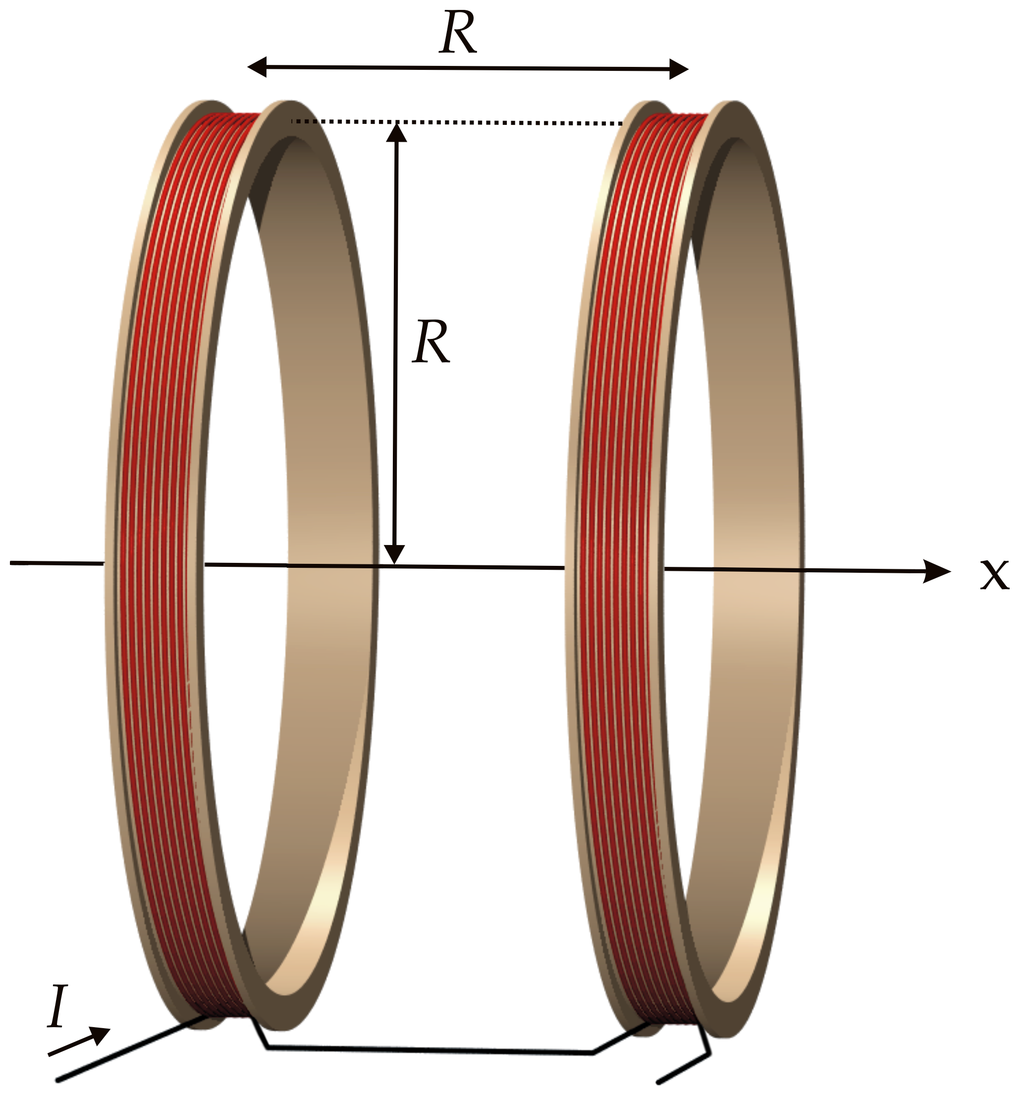
\includegraphics[width=0.8\linewidth]{pic/Helmholtz_coils}
		\caption{Схема котушок Гельмгольца (взято з \href{https://en.wikipedia.org/wiki/Helmholtz_coil}{wikipedia})}
		\label{pic:Helmholtz_coils}
	\end{minipage}
	\qquad%---------------------------------------------------------
	\begin{minipage}[t]{0.45\linewidth}\centering
		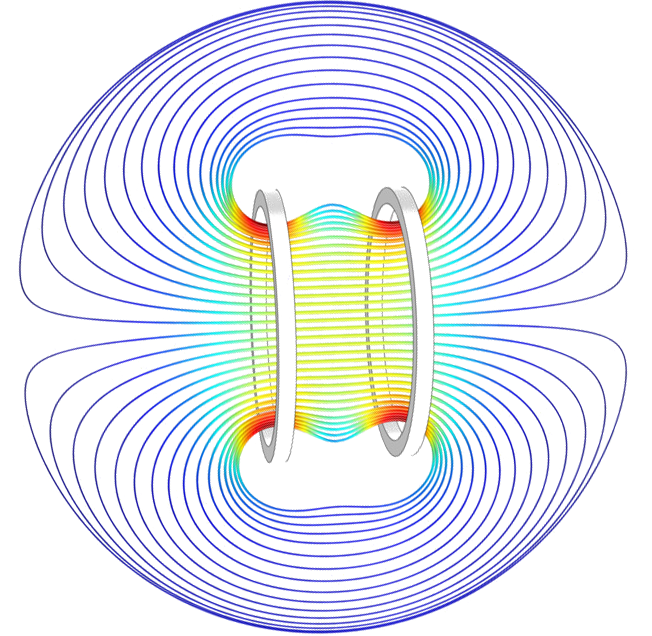
\includegraphics[width=0.8\linewidth]{pic/Helmholtz_coils_field}
		\caption{Вигляд поля котушок Гельмгольца (взято з \href{https://www.freepng.ru/png-d02278/}{https://www.freepng.ru/png-d02278/})}
		\label{pic:Helmholtz_coils_field}
	\end{minipage}
	%---------------------------------------------------------
\end{figure}
%=========================================================

Магнітне поле в центрі між котушками можна розрахувати за допомогою закону Біо-Савара-Лапласа, який дає формулу:
\begin{equation}\label{eq:Helmholtz_coils_field}
	B = \left( \frac45\right)^{\frac32} \frac{\mu_0 nI}{R}.
\end{equation}
Константою котушок називається величина $C = \frac{B}{I}$, яка, як випливає з~\eqref{eq:Helmholtz_coils_field} визначається формулою:
\begin{equation}\label{eq:Helmholtz_coils_constant}
	C = \left( \frac45\right)^{\frac32} \frac{\mu_0 n}{R},
\end{equation}
де $n$~--- кількість витків в одному кільці, $R$~--- радіус кільця.

\fputrue% ----- Увімкнення двигуна точних розрахунків
\pgfmathsetmacro{\muz}{4*pi*1e-7}
\pgfmathsetmacro{\R}{0.200}
\pgfmathsetmacro{\dR}{0.5e-2}
\pgfmathsetmacro{\n}{154}
\pgfmathsetmacro{\CG}{(4/5)^(3/2)*\muz*\n/\R}
\pgfmathsetmacro{\CGprint}{\CG*1e4}
\pgfmathsetmacro{\dCG}{(4/5)^(3/2)*\muz*\n/\R^2*\dR}
\pgfmathsetmacro{\dCGprint}{\dCG*1e4}
\fpufalse% ----- Вимкнення двигуна точних розрахунків

Для визначення константи, нам знадобиться вимірювати лише відстань $L$ між котушками, яка дорівнює їх радіусу за допомогою лінійки, тому треба визначити лише похибку прямого вимірювання $R$. Сама лінійка має дуже малу інструментальну похибку, однак зважаючи на те, що кільця складаються з багатьох витків, які поодинці знаходяться на відстанях дещо відмінних від $R$, що не враховано в формулі \eqref{eq:Helmholtz_coils_constant}, оцінимо систематичну похибку у вимірюванні відстані як $R = (\pgfmathprintnumber[fixed, fixed zerofill, precision=3]{\R} \pm \pgfmathprintnumber[fixed, fixed zerofill, precision=3]{\dR})$~м.

Похибку непрямого вимірювання константи ми визначимо як похибку непрямого вимірювання за формулою:
\begin{equation}\label{eq:Helmholtz_coils_constant2}
	\Delta C = \left( \frac45\right)^{\frac32} \frac{\mu_0 n}{R^2} \Delta R = \pgfmathprintnumber[]{\dCG}~\text{Тл/А},
\end{equation}

Таким чином, отримаємо результат:
\begin{equation}\label{}
	C_\text{БСЛ} =  (\pgfmathprintnumber[]{\CGprint} \pm \pgfmathprintnumber[]{\dCGprint})\cdot 10^{-4}~\text{Тл/А}.
\end{equation}

\begin{table}[h!]\small
	\centering
	\caption{Параметри котушок}
	\begin{tabular}{ll}
		\toprule
		\textbf{Величина}                & \textbf{Значення}                                                                               \\ \midrule
		Кількість витків в одному кільці & $N = \pgfmathprintnumber[]{\n}$                                                                 \\
		Радіус кільця                    & $R = \pgfmathprintnumber[fixed, fixed zerofill, precision=3]{\R}$ м                             \\ \midrule
		Похибка вимірюванні радіусу      & $\Delta R = \pgfmathprintnumber[fixed, fixed zerofill, precision=3]{\dR}$ м                     \\ \midrule
		Константа котушок                & $C =  (\pgfmathprintnumber[]{\CGprint} \pm \pgfmathprintnumber[]{\dCGprint})\cdot 10^{-4}$~Тл/А \\ \bottomrule
	\end{tabular}
	\label{tab:Helmgoltz_coils}
\end{table}

Далі виміряємо прямо залежність магнітного поля в центрі котушок, виміряну тесламетром від сили струму, що тече через котушки. Після обробки результатів, отримаємо графік зображений на рис.~\ref{fig2}.

\begin{Warning}
	Якщо з теорії відомо, що залежність між вимірюваними величинами є лінійною $y = ax + b$ і має проходити через початок координат, може виникнути бажання покласти $b = 0$. Проте, при початковому аналізі таких даних все одно краще цього не робити, оскільки це дозволить визначити систематичну похибку, яка може бути присутня в вимірюваннях (наприклад у приладу <<збитий нуль>>). Однак, якщо в результаті апроксимації виявиться, що $b \ll \Delta b$, то це означає, що параметр $b$ є надлишковим і в якості моделі можна прийняти  $y = ax$.
\end{Warning}

% ======= Завантаження данних для побудови ========
\pgfkeys{/pgf/fpu}
\pgfplotstableread[col sep = colon, header=false]{\outfile}\plotfitdata
\getelement{\plotfitdata}{0}{1}{\a} % Параметр моделі a
\getelement{\plotfitdata}{1}{1}{\da} % Стандартна похибка параметру a
\getelement{\plotfitdata}{2}{1}{\b} % Параметр моделі b
\getelement{\plotfitdata}{3}{1}{\db} % Стандартна похибка параметру b
\getelement{\plotfitdata}{4}{1}{\chisqr} % Приведений хі-квадрат
\getelement{\plotfitdata}{5}{1}{\rsq} % Коефіцієнт детермінації R^2
\pgfmathsetmacro{\aprint}{\a*1e4}
\pgfmathsetmacro{\daprint}{\da*1e4}
\pgfkeys{/pgf/fpu=false}

Результати мають наступний вигляд:
\begin{equation}\label{}
	C_\text{exp} = (\pgfmathprintnumber[precision=2, fixed, fixed zerofill]{\aprint} \pm \pgfmathprintnumber[precision=2, fixed, fixed zerofill]\daprint)\cdot 10^{-4}~\text{Тл/А},
\end{equation}

\begin{equation}\label{}
	\frac{\chi^2}{N-p} = \pgfmathprintnumber[precision=2,fixed]{\chisqr}.
\end{equation}
Критерій якості апроксимації, який дорівнює $\pgfmathprintnumber[precision=2,fixed]{\chisqr}$ і свідчить про те, що модель добре описується експериментом.

Порівняємо тепер результати двох вимірювань і вияснимо, наскільки вони співпадають. Для цього знайдемо різницю $|C_\text{БСЛ} - C_\text{exp}|$  і порівняємо її з похибкою експериментальних даних:
\pgfkeys{/pgf/fpu}
\pgfmathparse{abs(\CG - \a)/\da}
\pgfkeys{/pgf/fpu=false}

\begin{equation}
	\left|\frac{C_\text{БСЛ} - C_\text{exp}}{\Delta C}\right| \approx  \pgfmathprintnumber[precision=1,fixed, fixed zerofill]{\pgfmathresult}.
\end{equation}
Як видно відмінність двох значень становить $\pgfmathprintnumber[precision=1,fixed, fixed zerofill]{\pgfmathresult}$ стандартного відхилення, що з точки зору інтерпретації говорить, що ці величини однакові.

\begin{figure}[!hb]\centering
	\begin{tikzpicture}[trim axis left, trim axis right,]
		\begin{axis}[
				LabPlotGrid,
				enlargelimits=true,
				width=\linewidth,
				height=\linewidth,
				xlabel={$I$ / А},
				ylabel={$B$ / Тл},
				%				xtick scale label code/.code={$x$, $\cdot 10^{#1}$ м},
				scaled x ticks=base 10:0,
				%				ytick scale label code/.code={$y$, $\cdot 10^{#1}$ Н},
				scaled y ticks=base 10:4,
				xtick distance=0.2,
				title = {Калібрувальна крива котушок Гельмгольца},
				legend style={
						cells={anchor=west},
						legend pos=north west,
					},
			]
			% ================== Plot 1 =====================
			\addplot [only marks,
				mark options = {color = red},
				mark size = 2,
				error bars/.cd, y dir=both,
				x dir=both,
				y explicit,
				x explicit,
			] table[
					x = x,
					y = y,
					x error = xdelta,
					y error = ydelta] \datatable;
			\addlegendentry{Експериментальні дані}

			\addplot [no markers, blue, domain=0.9:2.3]  {
				\a * x
			};
			\addlegendentry{Лінійна апроксимація за моделлю $B = C \cdot I$}

			\node[anchor=south east, fill=white, align=left, draw, font=\sffamily] at ([shift ={(-0.25cm,0.25cm)}]current axis.south east) {
			$C = (\pgfmathprintnumber[precision=2, fixed, fixed zerofill]{\aprint} \pm \pgfmathprintnumber[precision=2, fixed, fixed zerofill]{\daprint})\cdot 10^{-4}$~Тл/А \\
			${\chi^2}/{\overline{\chi^2}} = \pgfmathprintnumber[precision=2,fixed]{\chisqr}$, $R^2 = \pgfmathprintnumber[precision=2,fixed]{\rsq}$ };
		\end{axis}
	\end{tikzpicture}
	\caption{Вимірювання залежності індукції магнітного поля $B$ в середині котушок Гельмгольца від сили струму $I$ в їх обмотках. Експериментальні дані та їх лінійна апроксимація. Наведено критерій якості апроксимації, який дорівнює $\pgfmathprintnumber[precision=2,fixed]{\chisqr}$ і свідчить про те, що модель добре описується експериментом}
	\label{fig2}
\end{figure}

\begin{Warning}
	Часто зустрічається помилка, коли студент знаходить кутовий коефіцієнт (параметр $a$) по середньому від частки. Наприклад, якщо вимірюється залежність  $B(I)$, то отримавши кілька експериментальних точок $(I_i, B_i)$, і користуючись формулою $C = \frac{B}{I}$, студент обчислює константу котушок для вимірювання $C_i = \frac{B_i}{I_i}$, а потім визначає саму константу як середнє значення
	\[
		\left\langle C \right\rangle = \frac1n \sum\limits_i C_i
	\]
	Помилки полягають в наступному: по-перше, застосовувати процедуру усереднення можна тільки при повторенні одного і того ж вимірювання. В даному випадку значення $C_i$ відносяться до різних вимірювань, так як параметри системи кожен раз змінювалися. По-друге, не можна перевірити, чи залежність дійсно лінійна. По-третє, навіть якщо залежність можна вважати лінійною, може виявитися так, що вона не проходить через нуль (наприклад, через зсув нуля амперметра або тесламетра) --- тоді формула $C_i = \frac{B_i}{I_i}$ не годиться. І нарешті, навіть якщо виконана лінійність і залежність проходить через нуль, обчислення таким способом загрожує великими похибками. Неважко бачити, що середнє значення $\left\langle \frac{B_i}{I_i} \right\rangle$ по суті є середнє тангенсів кутів нахилу ліній, проведених з початку координат в експериментальну точку. Як відомо, функція $\tg(x)$ при $x > \frac{\pi}{4}$ дуже різко зростає (і прямує до нескінченності при $\frac{\pi}{2}$). У такому випадку навіть невелике <<ворушіння>> експериментальної точки, особливо якщо вона знаходиться досить близько до осі ординат, може привести до різкого збільшення внеску цієї точки в підсумковий результат. Таким чином, <<розумний>> результат студента --- плід вдалого збігу багатьох обставин. Правильний --- обґрунтований і надійний--- алгоритм знаходження константи: побудувати графік $B(I)$, переконатися в його лінійності, і побудувати найкращу пряму. Кутовий коефіцієнт цієї прямої і буде найкращою оцінкою константи котушок Гельмгольца.
\end{Warning}


\clearpage
\section{Програмне забезпечення для апроксимації даних та побудови графіків. Приклади застосування}


Існує чимало програмних пакетів для апроксимації експериментальних даних. Зосередимось лише на потужному Open Source забезпеченні.
Нехай є експериментальні дані, подані у вигляді чотирьох колонок: самих даних \texttt{x}, \texttt{y}, та їх стандартних похибок \texttt{xdelta}, \texttt{ydelta}:

\bgroup
%    \captionof{listing}{Текстовий файл з даними\label{lst:Data}}
\inputminted[
	breaklines,
	fontsize=\small,
	fontfamily=tt,
	encoding=utf8,
	fontsize=\footnotesize,
	frame=lines,
	bgcolor=lightgray!20!white,
]{text}{ExpData.dat}
\egroup

Для цих даних необхідно перевірити модель $y = a x + b$, а також отримати параметр $a$ цієї моделі та його стандартну похибку $\Delta a$.


\subsection{Обробка результатів в \texttt{Python}}


В середовищі \texttt{Python} пакетом для чисельної обробки експериментальних даних є \href{https://scipy.org}{\texttt{scipy}}. Наведемо тут лише приклад виклику процедури оптимізації.

Для початку, треба завантажити дані в змінні:

%\captionof{listing}{Завантаження даних\label{lst:Data}}
\begin{minted}[
    breaklines,
    fontsize=\small,
    fontfamily=tt,
    encoding=utf8,
    fontsize=\footnotesize,
    frame=lines,
    bgcolor=lightgray!20!white,
]{python}
"""
Завантаження даних в змінні
"""
data = np.loadtxt(sys.argv[1], skiprows=1)
x = data[:, 0]
y = data[:, 1]
dx = data[:, 2]
dy = data[:, 3]
\end{minted}


Задаємо функцію, якою будемо апроксимувати наші дані:
\bgroup
%\captionof{listing}{Задаємо модельну функцію\label{lst:Model}}
\begin{minted}[
    breaklines,
    fontsize=\small,
    fontfamily=tt,
    encoding=utf8,
    fontsize=\footnotesize,
    frame=lines,
    bgcolor=lightgray!20!white,
]{python}
# Задаємо модельну функцію
def model_func(beta, x):
    """
    Визначення математичної моделі для підгони.

    Параметр підгонки beta[0] та beta[1]
    """
    y = beta[0] * x + beta[1]
    return y
\end{minted}
\egroup

Вибираємо метод \texttt{Orthogonal distance regression (ODR)} з бібліотеки \href{https://docs.scipy.org/doc/scipy/reference/odr.html}{\texttt{scipy.odr}}, який реалізує метод найменших повних квадратів, який і будемо використовувати для підгонки:
\bgroup
%\captionof{listing}{Задаємо модельну функцію\label{lst:Model}}
\begin{minted}[
    breaklines,
    fontsize=\small,
    fontfamily=tt,
    encoding=utf8,
    fontsize=\footnotesize,
    frame=lines,
    bgcolor=lightgray!20!white,
]{python}
# Створюємо екземпляр моделі
model = Model(model_func)

# Створюємо екземпляр даних data
data = RealData(x, y, dx, dy)

# Створюємо ODR зі своїми даними, моделлю та початковою оцінкою параметрів
odr = ODR(data, model, [6e-4, 0])

# Вибір методу підгонки
odr.set_job(fit_type=0)
\end{minted}
\egroup

Результати обробки даних програма вміщує в змінні. Параметр моделі --- \mintinline{python}{output.beta[0]}, стандартна похибка параметру моделі --- \mintinline{python}{output.beta[0]} та $\chi^2$ -- \mintinline{python}{output.res_var}. Після чого завдяки функції \mintinline{python}{np.savetxt} ці результати можна записати у файл.

\bgroup
%\captionof{listing}{Задаємо модельну функцію\label{lst:Model}}
\begin{minted}[
    breaklines,
    fontsize=\small,
    fontfamily=tt,
    encoding=utf8,
    fontsize=\footnotesize,
    frame=lines,
    bgcolor=lightgray!20!white,
]{python}
# Отримуємо результати підгонки
output = odr.run()

# Заапис параметрів у файл
np.savetxt(
    sys.argv[2],
    [
        ("Parameter", output.beta[0]),
        ("Standart Deviation", output.sd_beta[0]),
        ("chi square", output.res_var),
        ("R square", adjusted_Rsq),
    ],
    delimiter=": ",
    fmt="%s",
)
\end{minted}
\egroup

Повний лістинг скрипту (текст~\ref{lst:Full_Listing}). Скрипт отримує на вході файл з даними, а на виході записує файл з результатами апроксимації:
\bgroup
%\captionof{listing}{Задаємо модельну функцію\label{lst:Model}}
\begin{minted}[
    breaklines,
    fontsize=\small,
    fontfamily=tt,
    encoding=utf8,
    fontsize=\footnotesize,
    frame=lines,
    bgcolor=lightgray!20!white,
]{bash}
PyFit.py <file_with_experimental_data> <file_with_fit_parameters>
\end{minted}
\egroup

\bgroup
\captionof{listing}{Лістинг скрипта \texttt{PyFit.py}\label{lst:Full_Listing}}
\inputminted[
	linenos,
	breaklines,
	fontsize=\small,
	fontfamily=tt,
	encoding=utf8,
	fontsize=\footnotesize,
	frame=lines,
	bgcolor=lightgray!20!white,
]{python}{PyFit.py}
\egroup


\subsection{Обробка результатів в \texttt{Gnuplot}}


Ті ж самі обчислення можна зробити за допомогою \href{http://www.gnuplot.info}{\texttt{Gnuplot}}. Як сказано в  файлі \href{https://runebook.dev/en/docs/gnuplot/fit}{документації}, апроксимація даних здійснюється за алгоритмом описаним в статті~\cite{OREAR_LS}.

\bgroup
\captionof{listing}{Лістинг скрипта \texttt{GpFit.gp}\label{lst:Full_Listing_gp}}
\inputminted[
	linenos,
	breaklines,
	fontsize=\small,
	fontfamily=tt,
	encoding=utf8,
	fontsize=\footnotesize,
	frame=lines,
	bgcolor=lightgray!20!white,
]{Matlab}{GnuFit.gp}
\egroup


Скрипт отримує на вході файл з даними, а на виході записує файл з результатами апроксимації:
\bgroup
%\captionof{listing}{Задаємо модельну функцію\label{lst:Model}}
\begin{minted}[
    breaklines,
    fontsize=\small,
    fontfamily=tt,
    encoding=utf8,
    fontsize=\footnotesize,
    frame=lines,
    bgcolor=lightgray!20!white,
]{bash}
gnuplot -persist -c GnuFit.gp <file_with_experimental_data> <file_with_fit_parameters>
\end{minted}
\egroup

\begin{Warning}
	Слід зазначити, що існує величезна кількість засобів і способів оцінки оптимальних значень параметрів, тому при використанні того чи іншого інструменту, завжди слід читати документацію і з'ясовувати, що саме і як він виконує  алгоритм.

	Якщо поставити холіварне питання, що краще обирати \texttt{scipy}, \texttt{GnuPlot}, чи щось інше, то тут лише справа смаку. Деякі порівняння в роботі бібліотек \texttt{Python} та \texttt{GnuPlot}  можна знайти за посиланням \url{https://stackoverflow.com/a/23883352/4908648}.

	Також слід завжди перевіряти результати обробки з якісних міркувань.
\end{Warning}


\subsection{Побудова графіку за допомогою пакета \texttt{pgfplots/\LaTeX}}
Побудувати графік можна засобами того ж \texttt{Python} або \texttt{Gnuplot}, але набагато гнучкіше це можна зробити за допомогою пакета \texttt{pgfplots} для \LaTeX{}:

\bgroup
\captionof{listing}{Лістинг \texttt{\LaTeX} файлу\label{lst:pgfplots}}
\inputminted[
	linenos,
	breaklines,
	fontsize=\small,
	fontfamily=tt,
	encoding=utf8,
	fontsize=\footnotesize,
	frame=lines,
	bgcolor=lightgray!20!white,
]{latex}{ExpTreatPlt.tikz}
\egroup

\subsection{Апроксимація в \texttt{Google Colab}}

Ви також можете побачити роботу алгоритмів апроксимації в \texttt{Python} з використанням сервісу \href{https://colab.research.google.com/drive/11GaNT347aTwTcVdfJTYbV6nAh8TIRqMe?usp=sharing}{Google Colab}.

\nocite{*}
\printbibliography[heading=bibintoc, title=Перелік використаних джерел]

\end{document}
